\documentclass[]{book}
\usepackage{lmodern}
\usepackage{amssymb,amsmath}
\usepackage{ifxetex,ifluatex}
\usepackage{fixltx2e} % provides \textsubscript
\ifnum 0\ifxetex 1\fi\ifluatex 1\fi=0 % if pdftex
  \usepackage[T1]{fontenc}
  \usepackage[utf8]{inputenc}
\else % if luatex or xelatex
  \ifxetex
    \usepackage{mathspec}
  \else
    \usepackage{fontspec}
  \fi
  \defaultfontfeatures{Ligatures=TeX,Scale=MatchLowercase}
\fi
% use upquote if available, for straight quotes in verbatim environments
\IfFileExists{upquote.sty}{\usepackage{upquote}}{}
% use microtype if available
\IfFileExists{microtype.sty}{%
\usepackage{microtype}
\UseMicrotypeSet[protrusion]{basicmath} % disable protrusion for tt fonts
}{}
\usepackage{hyperref}
\hypersetup{unicode=true,
            pdftitle={Análisis multivariante de la comunidad},
            pdfauthor={Carlos Iván Espinosa},
            pdfborder={0 0 0},
            breaklinks=true}
\urlstyle{same}  % don't use monospace font for urls
\usepackage{natbib}
\bibliographystyle{apalike}
\usepackage{color}
\usepackage{fancyvrb}
\newcommand{\VerbBar}{|}
\newcommand{\VERB}{\Verb[commandchars=\\\{\}]}
\DefineVerbatimEnvironment{Highlighting}{Verbatim}{commandchars=\\\{\}}
% Add ',fontsize=\small' for more characters per line
\usepackage{framed}
\definecolor{shadecolor}{RGB}{248,248,248}
\newenvironment{Shaded}{\begin{snugshade}}{\end{snugshade}}
\newcommand{\KeywordTok}[1]{\textcolor[rgb]{0.13,0.29,0.53}{\textbf{{#1}}}}
\newcommand{\DataTypeTok}[1]{\textcolor[rgb]{0.13,0.29,0.53}{{#1}}}
\newcommand{\DecValTok}[1]{\textcolor[rgb]{0.00,0.00,0.81}{{#1}}}
\newcommand{\BaseNTok}[1]{\textcolor[rgb]{0.00,0.00,0.81}{{#1}}}
\newcommand{\FloatTok}[1]{\textcolor[rgb]{0.00,0.00,0.81}{{#1}}}
\newcommand{\ConstantTok}[1]{\textcolor[rgb]{0.00,0.00,0.00}{{#1}}}
\newcommand{\CharTok}[1]{\textcolor[rgb]{0.31,0.60,0.02}{{#1}}}
\newcommand{\SpecialCharTok}[1]{\textcolor[rgb]{0.00,0.00,0.00}{{#1}}}
\newcommand{\StringTok}[1]{\textcolor[rgb]{0.31,0.60,0.02}{{#1}}}
\newcommand{\VerbatimStringTok}[1]{\textcolor[rgb]{0.31,0.60,0.02}{{#1}}}
\newcommand{\SpecialStringTok}[1]{\textcolor[rgb]{0.31,0.60,0.02}{{#1}}}
\newcommand{\ImportTok}[1]{{#1}}
\newcommand{\CommentTok}[1]{\textcolor[rgb]{0.56,0.35,0.01}{\textit{{#1}}}}
\newcommand{\DocumentationTok}[1]{\textcolor[rgb]{0.56,0.35,0.01}{\textbf{\textit{{#1}}}}}
\newcommand{\AnnotationTok}[1]{\textcolor[rgb]{0.56,0.35,0.01}{\textbf{\textit{{#1}}}}}
\newcommand{\CommentVarTok}[1]{\textcolor[rgb]{0.56,0.35,0.01}{\textbf{\textit{{#1}}}}}
\newcommand{\OtherTok}[1]{\textcolor[rgb]{0.56,0.35,0.01}{{#1}}}
\newcommand{\FunctionTok}[1]{\textcolor[rgb]{0.00,0.00,0.00}{{#1}}}
\newcommand{\VariableTok}[1]{\textcolor[rgb]{0.00,0.00,0.00}{{#1}}}
\newcommand{\ControlFlowTok}[1]{\textcolor[rgb]{0.13,0.29,0.53}{\textbf{{#1}}}}
\newcommand{\OperatorTok}[1]{\textcolor[rgb]{0.81,0.36,0.00}{\textbf{{#1}}}}
\newcommand{\BuiltInTok}[1]{{#1}}
\newcommand{\ExtensionTok}[1]{{#1}}
\newcommand{\PreprocessorTok}[1]{\textcolor[rgb]{0.56,0.35,0.01}{\textit{{#1}}}}
\newcommand{\AttributeTok}[1]{\textcolor[rgb]{0.77,0.63,0.00}{{#1}}}
\newcommand{\RegionMarkerTok}[1]{{#1}}
\newcommand{\InformationTok}[1]{\textcolor[rgb]{0.56,0.35,0.01}{\textbf{\textit{{#1}}}}}
\newcommand{\WarningTok}[1]{\textcolor[rgb]{0.56,0.35,0.01}{\textbf{\textit{{#1}}}}}
\newcommand{\AlertTok}[1]{\textcolor[rgb]{0.94,0.16,0.16}{{#1}}}
\newcommand{\ErrorTok}[1]{\textcolor[rgb]{0.64,0.00,0.00}{\textbf{{#1}}}}
\newcommand{\NormalTok}[1]{{#1}}
\usepackage{longtable,booktabs}
\usepackage{graphicx,grffile}
\makeatletter
\def\maxwidth{\ifdim\Gin@nat@width>\linewidth\linewidth\else\Gin@nat@width\fi}
\def\maxheight{\ifdim\Gin@nat@height>\textheight\textheight\else\Gin@nat@height\fi}
\makeatother
% Scale images if necessary, so that they will not overflow the page
% margins by default, and it is still possible to overwrite the defaults
% using explicit options in \includegraphics[width, height, ...]{}
\setkeys{Gin}{width=\maxwidth,height=\maxheight,keepaspectratio}
\IfFileExists{parskip.sty}{%
\usepackage{parskip}
}{% else
\setlength{\parindent}{0pt}
\setlength{\parskip}{6pt plus 2pt minus 1pt}
}
\setlength{\emergencystretch}{3em}  % prevent overfull lines
\providecommand{\tightlist}{%
  \setlength{\itemsep}{0pt}\setlength{\parskip}{0pt}}
\setcounter{secnumdepth}{5}
% Redefines (sub)paragraphs to behave more like sections
\ifx\paragraph\undefined\else
\let\oldparagraph\paragraph
\renewcommand{\paragraph}[1]{\oldparagraph{#1}\mbox{}}
\fi
\ifx\subparagraph\undefined\else
\let\oldsubparagraph\subparagraph
\renewcommand{\subparagraph}[1]{\oldsubparagraph{#1}\mbox{}}
\fi

%%% Use protect on footnotes to avoid problems with footnotes in titles
\let\rmarkdownfootnote\footnote%
\def\footnote{\protect\rmarkdownfootnote}

%%% Change title format to be more compact
\usepackage{titling}

% Create subtitle command for use in maketitle
\providecommand{\subtitle}[1]{
  \posttitle{
    \begin{center}\large#1\end{center}
    }
}

\setlength{\droptitle}{-2em}

  \title{Análisis multivariante de la comunidad}
    \pretitle{\vspace{\droptitle}\centering\huge}
  \posttitle{\par}
    \author{Carlos Iván Espinosa}
    \preauthor{\centering\large\emph}
  \postauthor{\par}
      \predate{\centering\large\emph}
  \postdate{\par}
    \date{Octubre 2016}

\usepackage{booktabs}

\begin{document}
\maketitle

{
\setcounter{tocdepth}{1}
\tableofcontents
}
\chapter*{Prefacio}\label{prefacio}
\addcontentsline{toc}{chapter}{Prefacio}

\begin{center}\rule{0.5\linewidth}{\linethickness}\end{center}

La comunidad biológica se refiere a una agrupación de poblaciones de
especies que se presentan juntas en el espacio y el tiempo (Begon et al.
1999). Este concepto plantea que las comunidades tienen unos límites en
el espacio y el tiempo, y que estos límites están dados por la
distribución de las poblaciones. Sin embargo, la distribución de las
poblaciones no es homogénea y cada población responde diferente en el
espacio y el tiempo.

De esta forma la caracterización de una comunidad biológica se
constituye en un reto ya que implica poder rescatar los efectos que se
dan a varios niveles en la comunidad. El definir por ejemplo ¿Dónde
inicia y termina una comunidad? o ¿Cómo difieren las comunidades entre
localidades? o ¿Cómo la comunidad responde a las condiciones ambientales
o disturbios? representan algunas de las principales preguntas que
necesitamos responder. Una de las formas de responder estas preguntas
puede ser intentar cuantificar las similitudes entre localidades.

\chapter*{Objetivos}\label{objetivos}
\addcontentsline{toc}{chapter}{Objetivos}

\begin{center}\rule{0.5\linewidth}{\linethickness}\end{center}

\begin{itemize}
\item
  Comprender las bases teóricas para el cálculo de similitudes de la
  estructura de la comunidad entre localidades.
\item
  Utilizar herramientas de análisis para calcular índices de similitud y
  distancias entre comunidades.
\end{itemize}

\begin{figure}[htbp]
\centering
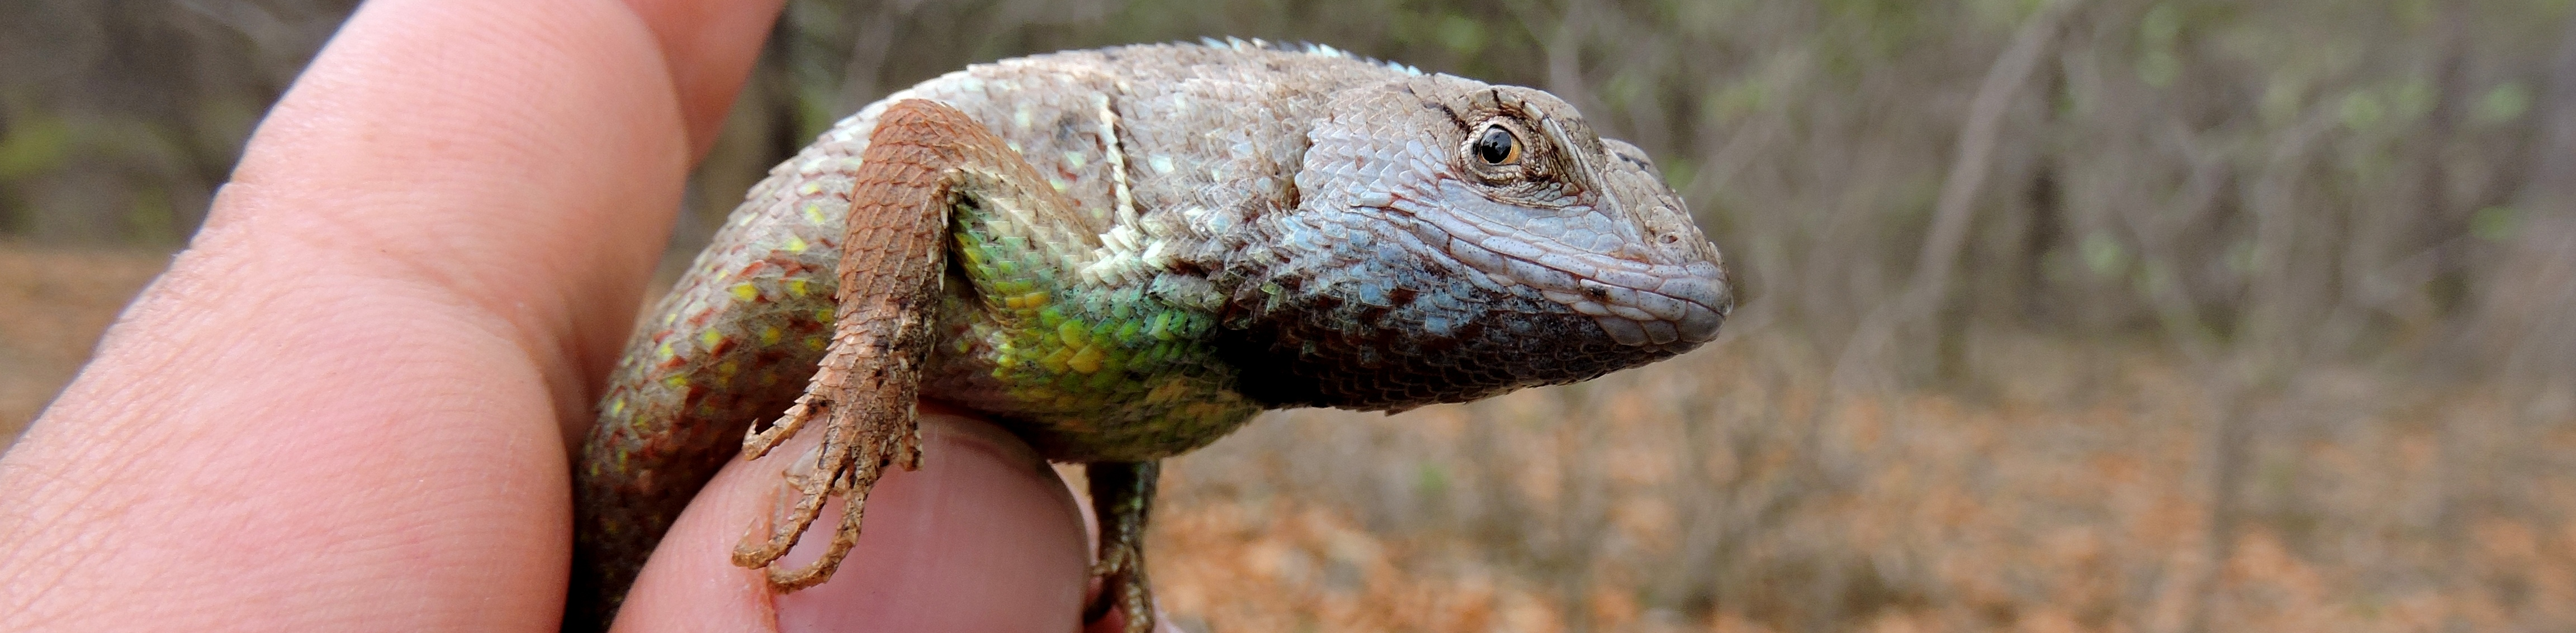
\includegraphics{lagar.jpg}
\caption{Stenocercus iridicens}
\end{figure}

\chapter{Análisis multivariado de la composición de la
comunidad}\label{analisis-multivariado-de-la-composicion-de-la-comunidad}

\begin{center}\rule{0.5\linewidth}{\linethickness}\end{center}

Los índices de similitud nos permiten comparar las comunidades entre dos
sitios, pero claramente cuando estudiamos las comunidades nuestros datos
no son tan sencillos como lo que hemos utilizado hasta el momento. El
organizar los datos de composición de la comunidad y poder
interpretarlos en relación a otras comunidades, entender que comunidades
son más similares entre sí, y saber si esta similitud o distancia es el
resultado de unas respuestas al entorno pueden ser algunas de las cosas
que podremos responder utilizando las técnicas de análisis multivariado
de la comunidad. A continuación vamos a describir algunas técnicas de
clasificación y ordenación que nos permitirán abordar estas temáticas.

Las técnicas de ordenación y clasificación son estrategias alternativas
para simplificar los datos. La ordenación intenta simplificar los datos
en un mapa que muestra las similitudes entre los puntos. La
clasificación simplifica datos colocando los puntos similares en una
misma clase o grupo Oksanen 2014\footnote{\url{http://cc.oulu.fi/~jarioksa/opetus/metodi/sessio3.pdf}}.

Utilizaremos el paquete \emph{Vegan} para los análisis de ordenación y
clasificación, para mayor información puede referirse a Oksanen
2013\footnote{\url{http://cc.oulu.fi/~jarioksa/opetus/metodi/vegantutor.pdf}}.

\section{Agrupamiento Jerárquico (Hierarchic
Cluster)}\label{agrupamiento-jerarquico-hierarchic-cluster}

A continuación vamos a realizar un análisis Cluster (análisis de
conglomerados) utilizando la función \emph{hclust} del paquete
\emph{vegan}. La función hclust necesita una matriz de disimilitudes
como entrada. El Análisis de conglomerados intenta generar conglomerados
que tengan la máxima homogeneidad en cada grupo y la mayor diferencia
entre los grupos.

Aunque la función \emph{dist} nos permite calcular disimilitudes, para
el análisis de comunidades biológicas utilizaremos la función
\emph{vegdist} del paquete \emph{vegan}. Esta función nos permite
calcular varios índices de disimilitud. El método de cálculo de la
disimilitud por defecto es Bray-Curtis (\emph{``bray''}).

Una de las características importantes del método Bray-Curtis es que
varía entre 0 y 1, dos comunidades que no comparten ninguna especie
tendrían 1 como resultado.

Calculemos una matriz de disimilitudes usando el método Bray-Curtis,
utilizaremos los datos de Barro Colorado Island (BCI) cargados en el
paquete \emph{vegan}. Para eso necesitamos cargar el paquete y los datos
de BCI, únicamente utilizaremos los datos de los primeros 10 sitios.

\begin{Shaded}
\begin{Highlighting}[]
\KeywordTok{library}\NormalTok{(vegan)}
\end{Highlighting}
\end{Shaded}

\begin{verbatim}
## Loading required package: permute
\end{verbatim}

\begin{verbatim}
## Loading required package: lattice
\end{verbatim}

\begin{verbatim}
## This is vegan 2.5-2
\end{verbatim}

\begin{Shaded}
\begin{Highlighting}[]
\KeywordTok{data}\NormalTok{(BCI)}

\NormalTok{dist<-}\StringTok{ }\KeywordTok{vegdist}\NormalTok{(BCI[}\DecValTok{1}\NormalTok{:}\DecValTok{10}\NormalTok{,], }\DataTypeTok{method=}\StringTok{"bray"}\NormalTok{)}
\NormalTok{dist[}\DecValTok{1}\NormalTok{:}\DecValTok{10}\NormalTok{]}
\end{Highlighting}
\end{Shaded}

\begin{verbatim}
##  [1] 0.2706682 0.3501647 0.3682008 0.3725079 0.3744186 0.3518519 0.3424346
##  [8] 0.4235706 0.3770140 0.2873051
\end{verbatim}

Podemos ver que el sitio 1 es 27\% diferente al sitio 2, 35\% al sitio
3, 36\% al sitio 4 y así sucesivamente con los 10 sitios.

Con la matriz de disimilitudes calculada se puede analizar los puntos
que conforman una agrupación. Utilizaremos los métodos de agrupación de
la función \emph{hclust} que nos propone tres métodos de agrupamiento:
agrupación simple, agrupación completa y agrupación promedio.

Todos los métodos inician con el agrupamiento de las dos comunidades
(dos sitios) más similares y a partir de esta primera comparación se
continúa con el resto de puntos.

A continuación ejemplificaremos el cálculo de las distancias usando los
tres métodos. Extraemos los cinco primeros sitios de la matriz de BCI y
generamos un nuevo objeto (S\_BCI). Con este nuevo objeto calculamos la
distancia entre los cinco sitios.

\begin{Shaded}
\begin{Highlighting}[]
\NormalTok{S_BCI<-}\StringTok{ }\NormalTok{BCI[}\DecValTok{1}\NormalTok{:}\DecValTok{5}\NormalTok{,]}
\NormalTok{dist1<-}\StringTok{ }\KeywordTok{vegdist}\NormalTok{(S_BCI, }\DataTypeTok{method=}\StringTok{"bray"}\NormalTok{)}
\NormalTok{dist1}
\end{Highlighting}
\end{Shaded}

\begin{verbatim}
##           1         2         3         4
## 2 0.2706682                              
## 3 0.3501647 0.2873051                    
## 4 0.3682008 0.3149523 0.3244078          
## 5 0.3725079 0.3851064 0.3595041 0.3721619
\end{verbatim}

\begin{enumerate}
\def\labelenumi{\arabic{enumi}.}
\item
  En base de la matriz de disimilitudes se busca el par de puntos que se
  encuentren más cercanos (menos disimiles). En nuestro caso el punto 1
  y 2 tienen la distancia más baja 0.27. Una vez identificado, inicia el
  proceso de agrupación y es donde se diferencian los tres métodos.
\item
  Con el primer grupo generado debemos comenzar la construcción del
  resto de grupos, para esto construimos una nueva matriz de disimilitud
  calculando las distancias desde este primer grupo (1-2) al resto de
  sitios. El cálculo de esta distancia es dependiente del método.
\end{enumerate}

\begin{quote}
Recuerde, para los sitios del 3 al 5 tendremos dos distancias, la
distancia desde el sitio 1 y del sitio 2 a cada uno de estos sitios. Por
tanto utilizaremos estas dos distancias para calcular la distancia desde
el grupo.
\end{quote}

\begin{itemize}
\tightlist
\item
  En el método de agrupación simple la distancia entre el grupo y el
  sitio 3 será igual a la distancia más baja comparando entre la
  distancia del sitio 1 y el sitio 2. En el caso de la distancia al
  sitio 3 el valor mínimo es 0.287.\\
\item
  En el método completo el nuevo valor de distancia será el valor más
  alto, en este caso 0.350, y
\item
  En el método de agrupación promedio, obtenemos el valor promedio entre
  las distancias primer grupo y el sitio 3 en este caso 0.318 (Tabla 1).
\end{itemize}

\textbf{Tabla 1.} Cálculo de nuevas distancias entre el grupo 1 (sitio 1
y 2) y los sitios restantes. \emph{\textbf{A. simple}}: cálculo de
distancia mediante el método de agrupación simple. \textbf{\emph{A.
completa}}: cálculo de distancia mediante el método de agrupación
completa. \textbf{\emph{A. promedio}}: cálculo de distancia mediante el
método de agrupación promedio.

\begin{longtable}[]{@{}llllll@{}}
\toprule
\begin{minipage}[b]{0.12\columnwidth}\raggedright\strut
Sitios\strut
\end{minipage} & \begin{minipage}[b]{0.14\columnwidth}\raggedright\strut
Sitio 1\strut
\end{minipage} & \begin{minipage}[b]{0.12\columnwidth}\raggedright\strut
Sitio 2\strut
\end{minipage} & \begin{minipage}[b]{0.15\columnwidth}\raggedright\strut
A. Simple\strut
\end{minipage} & \begin{minipage}[b]{0.17\columnwidth}\raggedright\strut
A. Completa\strut
\end{minipage} & \begin{minipage}[b]{0.14\columnwidth}\raggedright\strut
A. Media\strut
\end{minipage}\tabularnewline
\midrule
\endhead
\begin{minipage}[t]{0.12\columnwidth}\raggedright\strut
Sitio 3\strut
\end{minipage} & \begin{minipage}[t]{0.14\columnwidth}\raggedright\strut
0.3501647\strut
\end{minipage} & \begin{minipage}[t]{0.12\columnwidth}\raggedright\strut
0.2873051\strut
\end{minipage} & \begin{minipage}[t]{0.15\columnwidth}\raggedright\strut
0.2873051\strut
\end{minipage} & \begin{minipage}[t]{0.17\columnwidth}\raggedright\strut
0.3501647\strut
\end{minipage} & \begin{minipage}[t]{0.14\columnwidth}\raggedright\strut
0.3187349\strut
\end{minipage}\tabularnewline
\begin{minipage}[t]{0.12\columnwidth}\raggedright\strut
Sitio 4\strut
\end{minipage} & \begin{minipage}[t]{0.14\columnwidth}\raggedright\strut
0.3682008\strut
\end{minipage} & \begin{minipage}[t]{0.12\columnwidth}\raggedright\strut
0.3149523\strut
\end{minipage} & \begin{minipage}[t]{0.15\columnwidth}\raggedright\strut
0.3149523\strut
\end{minipage} & \begin{minipage}[t]{0.17\columnwidth}\raggedright\strut
0.3682008\strut
\end{minipage} & \begin{minipage}[t]{0.14\columnwidth}\raggedright\strut
0.3415765\strut
\end{minipage}\tabularnewline
\begin{minipage}[t]{0.12\columnwidth}\raggedright\strut
Sitio 5\strut
\end{minipage} & \begin{minipage}[t]{0.14\columnwidth}\raggedright\strut
0.3725079\strut
\end{minipage} & \begin{minipage}[t]{0.12\columnwidth}\raggedright\strut
0.3851064\strut
\end{minipage} & \begin{minipage}[t]{0.15\columnwidth}\raggedright\strut
0.3725079\strut
\end{minipage} & \begin{minipage}[t]{0.17\columnwidth}\raggedright\strut
0.3851064\strut
\end{minipage} & \begin{minipage}[t]{0.14\columnwidth}\raggedright\strut
0.3788071\strut
\end{minipage}\tabularnewline
\bottomrule
\end{longtable}

\begin{enumerate}
\def\labelenumi{\arabic{enumi}.}
\setcounter{enumi}{2}
\tightlist
\item
  A partir de estos cálculos se construye nuevamente la matriz de
  distancia. Mostramos las nuevas matrices de distancias según el método
  de agrupación utilizado.
\end{enumerate}

Para el método de agrupación \textbf{simple}

\begin{longtable}[]{@{}llll@{}}
\toprule
\begin{minipage}[b]{0.09\columnwidth}\raggedright\strut
Sitio\strut
\end{minipage} & \begin{minipage}[b]{0.15\columnwidth}\raggedright\strut
Grupo1-2\strut
\end{minipage} & \begin{minipage}[b]{0.14\columnwidth}\raggedright\strut
Sitio 3\strut
\end{minipage} & \begin{minipage}[b]{0.15\columnwidth}\raggedright\strut
Sitio 4\strut
\end{minipage}\tabularnewline
\midrule
\endhead
\begin{minipage}[t]{0.09\columnwidth}\raggedright\strut
3\strut
\end{minipage} & \begin{minipage}[t]{0.15\columnwidth}\raggedright\strut
0.2873051\strut
\end{minipage} & \begin{minipage}[t]{0.14\columnwidth}\raggedright\strut
\strut
\end{minipage} & \begin{minipage}[t]{0.15\columnwidth}\raggedright\strut
\strut
\end{minipage}\tabularnewline
\begin{minipage}[t]{0.09\columnwidth}\raggedright\strut
4\strut
\end{minipage} & \begin{minipage}[t]{0.15\columnwidth}\raggedright\strut
0.3149523\strut
\end{minipage} & \begin{minipage}[t]{0.14\columnwidth}\raggedright\strut
0.3244078\strut
\end{minipage} & \begin{minipage}[t]{0.15\columnwidth}\raggedright\strut
\strut
\end{minipage}\tabularnewline
\begin{minipage}[t]{0.09\columnwidth}\raggedright\strut
5\strut
\end{minipage} & \begin{minipage}[t]{0.15\columnwidth}\raggedright\strut
0.3725079\strut
\end{minipage} & \begin{minipage}[t]{0.14\columnwidth}\raggedright\strut
0.3595041\strut
\end{minipage} & \begin{minipage}[t]{0.15\columnwidth}\raggedright\strut
0.3721619\strut
\end{minipage}\tabularnewline
\bottomrule
\end{longtable}

Para el método de agrupación \textbf{completo}

\begin{longtable}[]{@{}llll@{}}
\toprule
\begin{minipage}[b]{0.09\columnwidth}\raggedright\strut
Sitio\strut
\end{minipage} & \begin{minipage}[b]{0.15\columnwidth}\raggedright\strut
Grupo1-2\strut
\end{minipage} & \begin{minipage}[b]{0.14\columnwidth}\raggedright\strut
Sitio 3\strut
\end{minipage} & \begin{minipage}[b]{0.15\columnwidth}\raggedright\strut
Sitio 4\strut
\end{minipage}\tabularnewline
\midrule
\endhead
\begin{minipage}[t]{0.09\columnwidth}\raggedright\strut
3\strut
\end{minipage} & \begin{minipage}[t]{0.15\columnwidth}\raggedright\strut
0.3501647\strut
\end{minipage} & \begin{minipage}[t]{0.14\columnwidth}\raggedright\strut
\strut
\end{minipage} & \begin{minipage}[t]{0.15\columnwidth}\raggedright\strut
\strut
\end{minipage}\tabularnewline
\begin{minipage}[t]{0.09\columnwidth}\raggedright\strut
4\strut
\end{minipage} & \begin{minipage}[t]{0.15\columnwidth}\raggedright\strut
0.3682008\strut
\end{minipage} & \begin{minipage}[t]{0.14\columnwidth}\raggedright\strut
0.3244078\strut
\end{minipage} & \begin{minipage}[t]{0.15\columnwidth}\raggedright\strut
\strut
\end{minipage}\tabularnewline
\begin{minipage}[t]{0.09\columnwidth}\raggedright\strut
5\strut
\end{minipage} & \begin{minipage}[t]{0.15\columnwidth}\raggedright\strut
0.3851064\strut
\end{minipage} & \begin{minipage}[t]{0.14\columnwidth}\raggedright\strut
0.3595041\strut
\end{minipage} & \begin{minipage}[t]{0.15\columnwidth}\raggedright\strut
0.3721619\strut
\end{minipage}\tabularnewline
\bottomrule
\end{longtable}

Para el método de agrupación \textbf{promedio}

\begin{longtable}[]{@{}llll@{}}
\toprule
\begin{minipage}[b]{0.09\columnwidth}\raggedright\strut
Sitio\strut
\end{minipage} & \begin{minipage}[b]{0.15\columnwidth}\raggedright\strut
Grupo1-2\strut
\end{minipage} & \begin{minipage}[b]{0.14\columnwidth}\raggedright\strut
Sitio 3\strut
\end{minipage} & \begin{minipage}[b]{0.15\columnwidth}\raggedright\strut
Sitio 4\strut
\end{minipage}\tabularnewline
\midrule
\endhead
\begin{minipage}[t]{0.09\columnwidth}\raggedright\strut
3\strut
\end{minipage} & \begin{minipage}[t]{0.15\columnwidth}\raggedright\strut
0.3187349\strut
\end{minipage} & \begin{minipage}[t]{0.14\columnwidth}\raggedright\strut
\strut
\end{minipage} & \begin{minipage}[t]{0.15\columnwidth}\raggedright\strut
\strut
\end{minipage}\tabularnewline
\begin{minipage}[t]{0.09\columnwidth}\raggedright\strut
4\strut
\end{minipage} & \begin{minipage}[t]{0.15\columnwidth}\raggedright\strut
0.3415765\strut
\end{minipage} & \begin{minipage}[t]{0.14\columnwidth}\raggedright\strut
0.3244078\strut
\end{minipage} & \begin{minipage}[t]{0.15\columnwidth}\raggedright\strut
\strut
\end{minipage}\tabularnewline
\begin{minipage}[t]{0.09\columnwidth}\raggedright\strut
5\strut
\end{minipage} & \begin{minipage}[t]{0.15\columnwidth}\raggedright\strut
0.3788071\strut
\end{minipage} & \begin{minipage}[t]{0.14\columnwidth}\raggedright\strut
0.3595041\strut
\end{minipage} & \begin{minipage}[t]{0.15\columnwidth}\raggedright\strut
0.3721619\strut
\end{minipage}\tabularnewline
\bottomrule
\end{longtable}

\begin{enumerate}
\def\labelenumi{\arabic{enumi}.}
\setcounter{enumi}{3}
\tightlist
\item
  Se repite el procedimiento, se busca los puntos que tienen la menor
  disimilitud en la nueva matriz y se vuelve a calcular las distancias
  desde este nuevo grupo al resto de grupos, esto se repite tantas veces
  hasta que todos los sitios están asociados.
\end{enumerate}

Podemos calcular directamente la agrupación utilizando la función
\emph{hclust}, y graficarlo con la función \emph{plot}.

\begin{Shaded}
\begin{Highlighting}[]
\KeywordTok{par}\NormalTok{(}\DataTypeTok{mfcol=}\KeywordTok{c}\NormalTok{(}\DecValTok{1}\NormalTok{,}\DecValTok{3}\NormalTok{))}

\NormalTok{csim <-}\StringTok{ }\KeywordTok{hclust}\NormalTok{(dist1, }\DataTypeTok{method=}\StringTok{"single"}\NormalTok{)}
\NormalTok{ccom <-}\StringTok{ }\KeywordTok{hclust}\NormalTok{(dist1, }\DataTypeTok{method=}\StringTok{"complete"}\NormalTok{)}
\NormalTok{cpro <-}\StringTok{ }\KeywordTok{hclust}\NormalTok{(dist1, }\DataTypeTok{method=}\StringTok{"average"}\NormalTok{)}

\KeywordTok{plot}\NormalTok{(csim, }\DataTypeTok{cex.axis=}\FloatTok{0.7}\NormalTok{)}
\KeywordTok{plot}\NormalTok{(ccom, }\DataTypeTok{cex.axis=}\FloatTok{0.7}\NormalTok{)}
\KeywordTok{plot}\NormalTok{(cpro, }\DataTypeTok{cex.axis=}\FloatTok{0.7}\NormalTok{)}
\end{Highlighting}
\end{Shaded}

\begin{figure}[htbp]
\centering
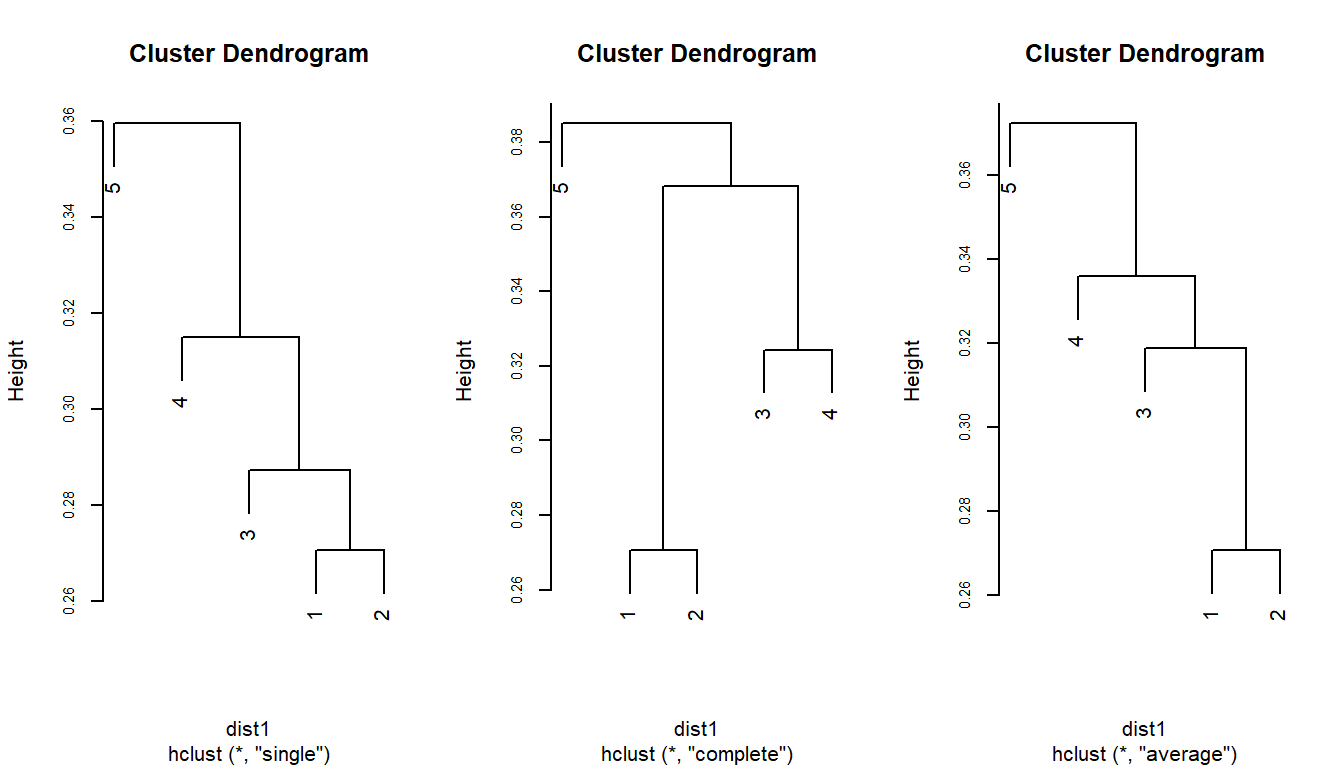
\includegraphics{AnalisisMultivarianteComunidad_files/figure-latex/den3-1.pdf}
\caption{\label{fig:den3}Dendrograma construido a partir de los 3 métodos de
agrupación}
\end{figure}

Como podemos ver en la figura \ref{fig:den3} en todos los casos el
primer grupo es el mismo, el grupo entre los sitios 1 y 2 con una
disimilitud de 0.27, a partir de este punto los dendrogramas varían
según el método utilizado. En el caso del método simple la disimilitud
más baja es entre el grupo 1-2 y el sitio 3, con una disimilitud del
0.287. En el caso del método completo la disimilitud más baja se da
entre el sitio 3 y 4 que conforman un segundo grupo con una disimilitud
de 0.32. Finalmente, en el caso del método de promedio la menor
disimilitud se da entre el grupo 1-2 y el sitio 3 con una disimilitud de
0.31 (Figura \ref{fig:den3})

Los métodos de agrupamiento jerárquico (cluster) producen
clasificaciones donde todas las observaciones se encuentran agrupadas de
diferente forma. En los extremos todas las observaciones se encuentran
agrupadas en una sola clase o cada observación conforma su clase
privada, entre estos extremos las observaciones forman diferentes
agrupamientos con niveles de disimilitud variables. Normalmente nos
interesa tener un cierto número de clases con niveles de disimilitud
establecido. La conformación de estos grupos se puede mostrar
visualmente con función \textbf{rect.hclust} (Figura \ref{fig:dengr})

\begin{Shaded}
\begin{Highlighting}[]
\KeywordTok{par}\NormalTok{(}\DataTypeTok{mar=}\KeywordTok{c}\NormalTok{(}\DecValTok{2}\NormalTok{,}\DecValTok{3}\NormalTok{,}\DecValTok{4}\NormalTok{,}\DecValTok{2}\NormalTok{))}
\KeywordTok{plot}\NormalTok{(ccom, }\DataTypeTok{hang=}\NormalTok{-}\FloatTok{0.1}\NormalTok{, }\DataTypeTok{cex.axis=}\FloatTok{0.7}\NormalTok{, }\DataTypeTok{cex.lab=}\FloatTok{0.8}\NormalTok{, }\DataTypeTok{cex.main=}\FloatTok{0.8}\NormalTok{)}
\KeywordTok{rect.hclust}\NormalTok{(ccom, }\DecValTok{3}\NormalTok{)}
\end{Highlighting}
\end{Shaded}

\begin{figure}[htbp]
\centering
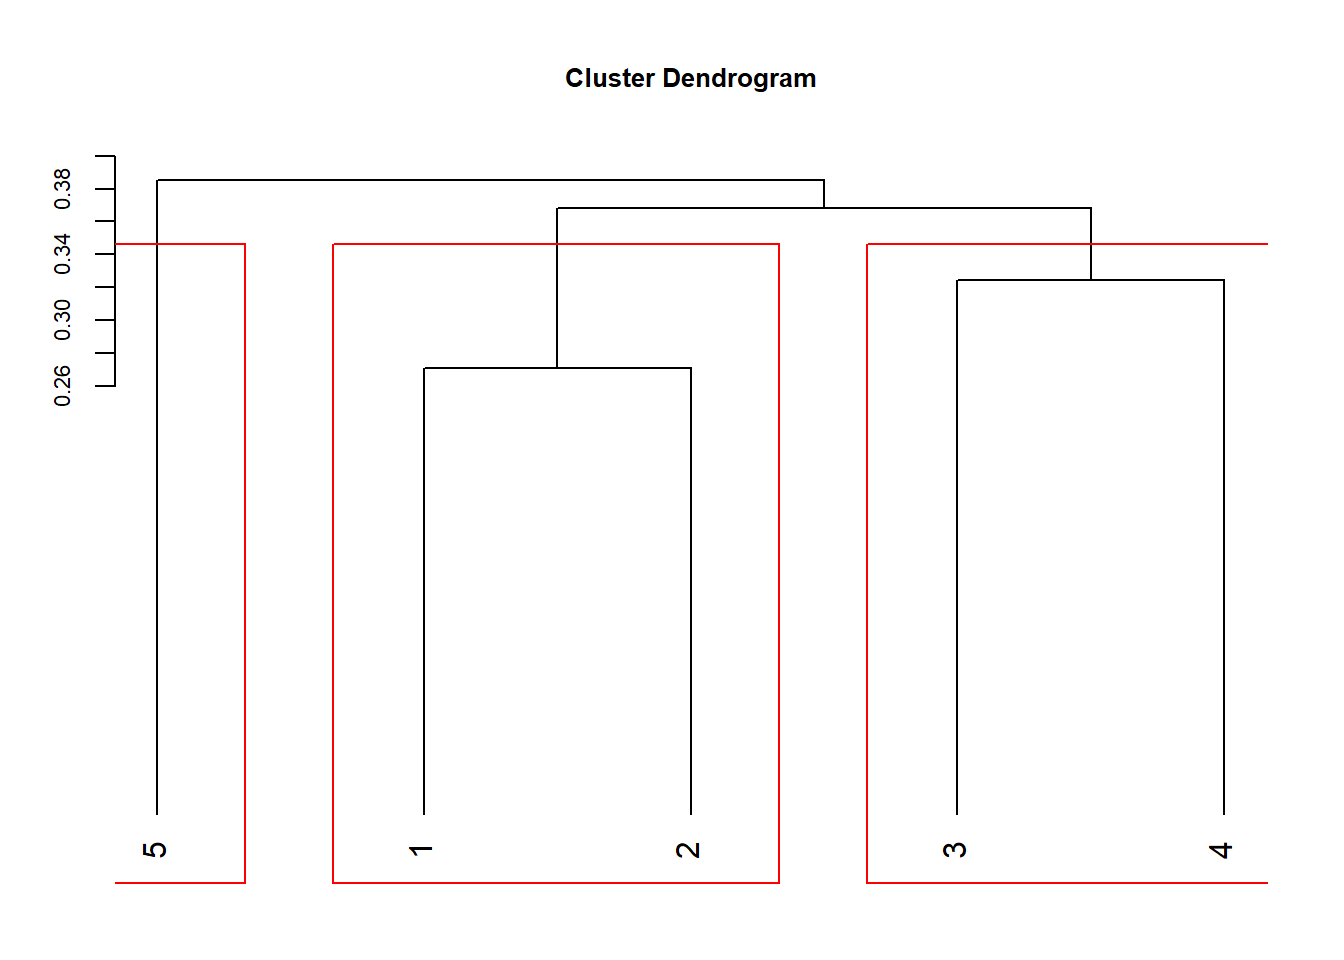
\includegraphics{AnalisisMultivarianteComunidad_files/figure-latex/dengr-1.pdf}
\caption{\label{fig:dengr}Dendrograma con número de grupos}
\end{figure}

Ahora podríamos obtener la pertenencia a un grupo y relacionarlo con
otra variable explicativa, y analizar si la genración del grupo responde
a algún factor.

\begin{Shaded}
\begin{Highlighting}[]
\NormalTok{grupo <-}\StringTok{ }\KeywordTok{cutree}\NormalTok{(ccom, }\DecValTok{3}\NormalTok{)}
\NormalTok{grupo}
\end{Highlighting}
\end{Shaded}

\begin{verbatim}
## 1 2 3 4 5 
## 1 1 2 2 3
\end{verbatim}

\section{Interpretando el cluster}\label{interpretando-el-cluster}

El análisis de conglomerados (cluster) no es un test estadístico, y como
vimos hay varios factores que pueden afectar la generación de los grupos
\citep{Borcard2011}, por lo que debemos ser consientes de lo que
obtenemos como resultado. POdemos usar la función \texttt{summary()}
para ver la información que tenemos luego de haber utilizado el
\texttt{hclust}, estos datos pueden ser utilizados para interpretar el
agrupamiento \citep{Borcard2011}.

Como vimos anteriormente el investigador puede decidir, en función de su
experiencia y de los arboles generados, cuantos grupos se generan dentro
del árbol y que metodo de agrupamiento utilizar, sin embargo, podemos
utilizar algunas funciones que nos permitan determinar grupos
consistentes.

\subsection{Elegir la función de
enlace}\label{elegir-la-funcion-de-enlace}

Una forma que podemos utilizar para definir los grupos es la distancia
Cofenética. Esta distancia es calculada como la distancia entre dos
objetos de un mismo grupo en el dendrograma, la distancia desde el
primer objeto al segundo objeto pasando por el nodo de unión de los dos
objetos es la distancia Cofenética. Una matriz cofenética es una matriz
que representa las distancias cophenéticas entre todos los pares de
objetos. Con esta matriz podemos correlacionar con la matriz de
disimilitud original. El método con la correlación cofenética más alta
puede ser vista como la que produjo el mejor modelo de agrupación para
la matriz de distancia.

\begin{Shaded}
\begin{Highlighting}[]
\CommentTok{#Calculamos la matriz cofenética para cada método de}
\CommentTok{#agrupamiento}

\NormalTok{csim_coph <-}\StringTok{ }\KeywordTok{cophenetic}\NormalTok{(csim)}
\NormalTok{cpro_coph <-}\StringTok{ }\KeywordTok{cophenetic}\NormalTok{(cpro)}
\NormalTok{ccom_coph <-}\StringTok{ }\KeywordTok{cophenetic}\NormalTok{(ccom)}

\CommentTok{#Calculamos la correlación}
\KeywordTok{cor}\NormalTok{(csim_coph, dist1); }\KeywordTok{cor}\NormalTok{(cpro_coph, dist1);}\KeywordTok{cor}\NormalTok{(ccom_coph, dist1)}
\end{Highlighting}
\end{Shaded}

\begin{verbatim}
## [1] 0.8143114
\end{verbatim}

\begin{verbatim}
## [1] 0.846916
\end{verbatim}

\begin{verbatim}
## [1] 0.7487461
\end{verbatim}

Según estos datos el método promedio es el método que produce un mejor
agrupamiento.

Otra forma de evaluar el mejor método es calcular la distancia de Gower,
calculado como la suma de los cuadrados de la diferencia entre la matriz
de distancia y la distancia Cofenética, el menor valor significa que es
el mejor método de agrupamiento.

\begin{Shaded}
\begin{Highlighting}[]
\NormalTok{sim_gow <-}\StringTok{ }\KeywordTok{sum}\NormalTok{((dist1-csim_coph)^}\DecValTok{2}\NormalTok{)}
\NormalTok{pro_gow <-}\StringTok{ }\KeywordTok{sum}\NormalTok{((dist1-cpro_coph)^}\DecValTok{2}\NormalTok{)}
\NormalTok{com_gow <-}\StringTok{ }\KeywordTok{sum}\NormalTok{((dist1-ccom_coph)^}\DecValTok{2}\NormalTok{)}

\NormalTok{sim_gow; pro_gow; com_gow}
\end{Highlighting}
\end{Shaded}

\begin{verbatim}
## [1] 0.007860928
\end{verbatim}

\begin{verbatim}
## [1] 0.003917673
\end{verbatim}

\begin{verbatim}
## [1] 0.01068659
\end{verbatim}

En este caso vemos que la decisión usando la distancia de Gower y la
Cofenética es la misma, el método promedio produce el mejor
agrupamiento. Sin embargo, no siempre el resultado es consistente entre
los dos métodos.

\begin{quote}
Este proceso nos ha permitido obtener la mejor función de enlace, sin
embargo, para definir cuales son los subconjuntos de datos (tener un
punto de corte) se puede utilizar algunas otras herramientas.
\end{quote}

\subsection{Elegir el punto de corte}\label{elegir-el-punto-de-corte}

Como vimos anteriormente yo puedo definir un punto de corte para generar
los grupos o puedo decidir cuantos grupos, sin embargo, este
procedimiento es subjetivo. Podemos utilizar alguna información que nos
permita tomar decisiones fundamentadas.

Podemos utilizar la \textbf{silhouette width (anchura de la silueta)}
para medir el grado de pertenencia de un objeto a su agrupación, basado
en la distancia media entre este objeto y todos los objetos de la
agrupación a la que se pertenece, en comparación con la misma medida
calculada para el siguiente grupo más cercano \citep{Borcard2011}.
Utilizaremos la función \texttt{siluette} del paquete \textbf{cluster}.
La salida de esta función varía entre 1 y -1. Los valores negativos
significan que los objetos correspondientes probablemente se han
colocado en un grupo erróneo.

A continuación el proceso utilizado:

\begin{Shaded}
\begin{Highlighting}[]
\KeywordTok{library}\NormalTok{(cluster)}

\CommentTok{#Generamos un vector vacío para colocar los valores }
\CommentTok{# medios de la anchura de la silueta (mas)}
\NormalTok{mas <-}\StringTok{ }\KeywordTok{numeric}\NormalTok{(}\KeywordTok{nrow}\NormalTok{(S_BCI))}

\CommentTok{#Calculamos y ponemos el <mas> en el vector generado}
\NormalTok{for( k in }\DecValTok{2}\NormalTok{:}\StringTok{ }\NormalTok{(}\KeywordTok{nrow}\NormalTok{(S_BCI)-}\DecValTok{1}\NormalTok{))\{}
    \NormalTok{sil <-}\StringTok{ }\KeywordTok{silhouette}\NormalTok{(}\KeywordTok{cutree}\NormalTok{(ccom, }\DataTypeTok{k=}\NormalTok{k), dist1)}
  \NormalTok{mas[k] <-}\StringTok{ }\KeywordTok{summary}\NormalTok{(sil)$avg.width}
\NormalTok{\}}

\CommentTok{# Analizamos cual es el mejor punto de corte}
\NormalTok{k.best <-}\StringTok{ }\KeywordTok{which.max}\NormalTok{(mas)}

\CommentTok{# Graficamos}
\KeywordTok{plot}\NormalTok{(}\DecValTok{1}\NormalTok{:}\KeywordTok{nrow}\NormalTok{(S_BCI), mas, }\DataTypeTok{type =} \StringTok{"h"}\NormalTok{, }\DataTypeTok{main=}\StringTok{"Número de grupos óptimo"}\NormalTok{, }
     \DataTypeTok{xlab =} \StringTok{"Número de grupos (k)"}\NormalTok{, }\DataTypeTok{ylab=}\StringTok{"Media de la anchura de la silueta"}\NormalTok{)}
\KeywordTok{axis}\NormalTok{(}\DecValTok{1}\NormalTok{, k.best, }\KeywordTok{paste}\NormalTok{(}\StringTok{"Optimo"}\NormalTok{, k.best, }\DataTypeTok{sep=}\StringTok{"}\CharTok{\textbackslash{}n}\StringTok{"}  \NormalTok{), }
     \DataTypeTok{col=}\StringTok{"red"}\NormalTok{, }\DataTypeTok{font=}\DecValTok{2}\NormalTok{, }\DataTypeTok{col.axis=}\StringTok{"red"}\NormalTok{)}
\KeywordTok{points}\NormalTok{(k.best, }\KeywordTok{max}\NormalTok{(mas), }\DataTypeTok{pch=}\DecValTok{16}\NormalTok{, }\DataTypeTok{col=}\StringTok{"red"}\NormalTok{, }\DataTypeTok{cex=}\FloatTok{1.5}\NormalTok{)}
\end{Highlighting}
\end{Shaded}

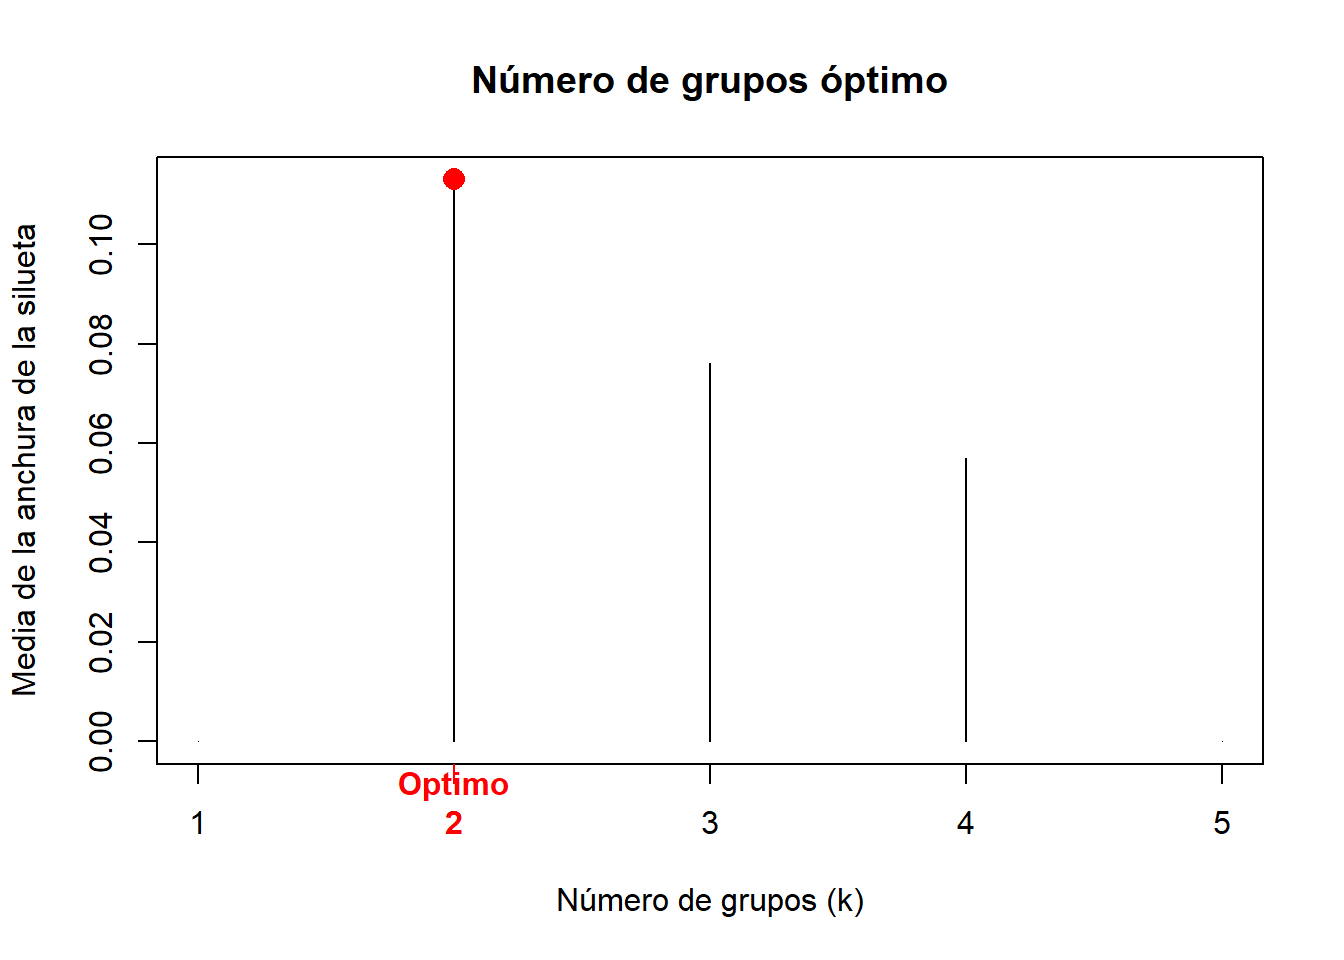
\includegraphics{AnalisisMultivarianteComunidad_files/figure-latex/unnamed-chunk-6-1.pdf}

\begin{Shaded}
\begin{Highlighting}[]
\KeywordTok{cat}\NormalTok{(}\StringTok{""}\NormalTok{, }\StringTok{"Número óptimo de grupos k="}\NormalTok{, k.best, }\StringTok{"}\CharTok{\textbackslash{}n}\StringTok{"}\NormalTok{,}
    \StringTok{"Con un valor medio de anchura de la silueta de"}\NormalTok{, }\KeywordTok{max}\NormalTok{(mas), }\StringTok{"}\CharTok{\textbackslash{}n}\StringTok{"}\NormalTok{)}
\end{Highlighting}
\end{Shaded}

\begin{verbatim}
##  Número óptimo de grupos k= 2 
##  Con un valor medio de anchura de la silueta de 0.1130222
\end{verbatim}

A partir de este punto podría utilizar otras herramientas para definir
el número de grupos. Ahora nos interesa saber si los grupos están
balanceados y bien delimitados. Podemos utilizar el gráfico de la
silueta

\begin{Shaded}
\begin{Highlighting}[]
\NormalTok{k<-}\StringTok{ }\DecValTok{2}
\NormalTok{cutg <-}\StringTok{ }\KeywordTok{cutree}\NormalTok{(ccom, }\DataTypeTok{k=}\NormalTok{k)}
\NormalTok{sil <-}\StringTok{ }\KeywordTok{silhouette}\NormalTok{(cutg, dist1)}
\NormalTok{sil.o <-}\StringTok{ }\KeywordTok{sortSilhouette}\NormalTok{(sil)}

\KeywordTok{rownames}\NormalTok{(sil.o) <-}\StringTok{ }\KeywordTok{row.names}\NormalTok{(S_BCI)[}\KeywordTok{attr}\NormalTok{(sil.o, }\StringTok{"iOrd"}\NormalTok{)]}

\KeywordTok{plot}\NormalTok{(sil.o, }\DataTypeTok{main=} \StringTok{"Gráfico de silueta"}\NormalTok{, }\DataTypeTok{cex.names =} \FloatTok{0.8}\NormalTok{, }
     \DataTypeTok{col =} \NormalTok{cutg}\DecValTok{+3}\NormalTok{, }\DataTypeTok{nmax.lab=}\DecValTok{100}\NormalTok{)}
\end{Highlighting}
\end{Shaded}

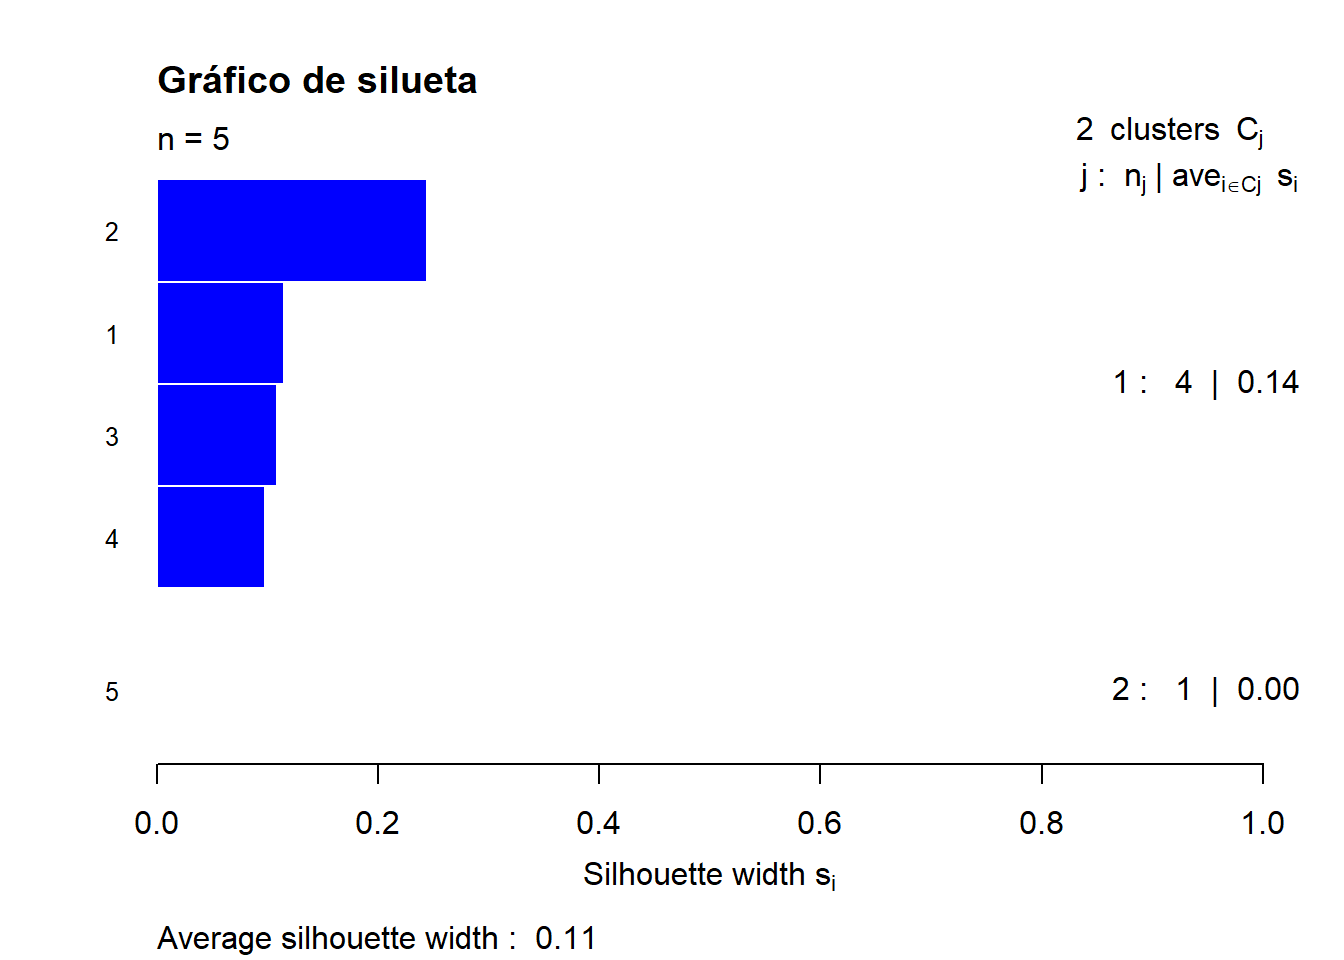
\includegraphics{AnalisisMultivarianteComunidad_files/figure-latex/unnamed-chunk-7-1.pdf}

Al parecer no ha sido el mejor ejemplo, sin embargo, podemos ver que los
2 grupos han sido consistentes. Vamos a probar con nuevos datos.

\section{ANOSIM\ldots{}Incluir}\label{anosimincluir}

\section{Ejercicio 2: Análisis de
clasificación}\label{ejercicio-2-analisis-de-clasificacion}

Con el fin de determinar si existen agrupamientos de herbaceas dentro de
una parcela permanente de 9ha en la Reserva Ecológica Arenillas
realizaremos un análisis de Agrupamiento (Cluster).

Para esto disponemos de una matriz con datos de la composición de la
comunidad que puede ser descargado
\href{https://github.com/Ciespinosa/datos_practicas/blob/master/herbaceas.xlsx}{aquí}.

Los datos corresponden a un levantamiento de la vegetación de herbáceas
en 4 tiempos distintos; final de invierno (abril 2012), estación seca
(noviembre 2012), inicio del invierno (diciembre 2012), invierno (enero
2013). Se levantaron 4 cuadrantes de 0.5x0.5 m en cada vértice y centro
de la parcela permanente de 9 hectáreas (113 muestras).

Con estos datos:

\begin{enumerate}
\def\labelenumi{\arabic{enumi}.}
\item
  Calcular una matriz de disimilitud utilizando la distancia de
  Bray-Curtis.
\item
  Definir la mejor función de enlace para los tres métodos.
\item
  Definir usando la función silhouette cuantos grupos deberían
  generarse.
\item
  Realizar un gráfico del cluster y mostrar los grupos con la función
  rect.hclust
\item
  Evaluar si los grupos obtenidos responden a alguna de las variables de
  especies leñosas
\item
  Graficar las coordenadas \textbf{``x''} y \textbf{``y''} de las
  parcelas y colorear cada punto de acuerdo al grupo al que pertenece.
  Esto nos permitirá identificar si existe un patrón espacial en la
  generación de los grupos.
\end{enumerate}

\chapter{Ordenaciones}\label{ordenaciones}

En ecología es bastante normal que dispongamos de datos que están
conformados por un conjunto de sitios o localidades, para los cuales
tenemos una serie de variables. Estas variables puede ser cada especie o
cada condición que levantemos en el sitio, de esta forma, un sitio va a
tener tantas variables como especies o factores ambientales se
registren.

En el capítulo de
\href{https://ciespinosa.github.io/Similitud/index.html}{similitud}
ordenamos las parcelas en función de la cantidad de individuos de dos
especies, de esta forma la distancia a la que se encontraba cada
comunidad nos daba información sobre cuanto se parecían. Aunque esta es
una forma fácil de \textbf{ordenar} nuestras comunidades, esta forma de
graficar es solo posible con dos o máximo tres especies, pero pocas
comunidades tienen únicamente tres especies, cuando tenemos más de tres
especies es necesario buscar otras formas de ordenación que nos permitan
rescatar el gradiente ambiental.

De esta forma, el objetivo de los métodos de ordenación es representar
los datos a lo largo de un número reducido de ejes ortogonales,
construidos de tal manera que representan, en orden, las principales
tendencias de los datos \citep{Borcard2011}.

Las ordenaciones pueden ser indirectas y directas (constreñidas). Las
ordenaciones indirectas pueden ser utilizadas para interpretarse
visualmente o asociadas a otros métodos, como regresión. Por su parte,
las ordenaciones directas permiten hacer asociaciones con variables
explicativas, generando un orden constreñido pobasado en unas variables
explicativas.

\section{Pasos previos a la
Ordenación}\label{pasos-previos-a-la-ordenacion}

\textbf{1. Decidir qué ordenación realizar}

Dentro de las ordenaciones directas e indirectas, existen muchos tipos
de ordenaciones ¿Cómo saber qué ordenación debo utilizar? Una
posibilidad es ver el tipo de respuesta de nuestros datos, si es una
respuesta lineal (monotónica) o una respuesta unimodal (distribución en
campana).

Una forma para determinar el tipo de respuesta de nuestros datos, es
asumir una distribución normal y usar la desviación estándar como una
medida del tipo de respuesta. Si nuestros datos tienen una dispersión
con menos de tres desviaciones estándar, podremos asumir que nuestros
datos tendrán una respuesta lineal (Figura \ref{fig:resp}a), mientras
que si tiene más de tres desviaciones se asumirá una respuesta unimodal
(Figura \ref{fig:resp}b).

\begin{figure}[htbp]
\centering
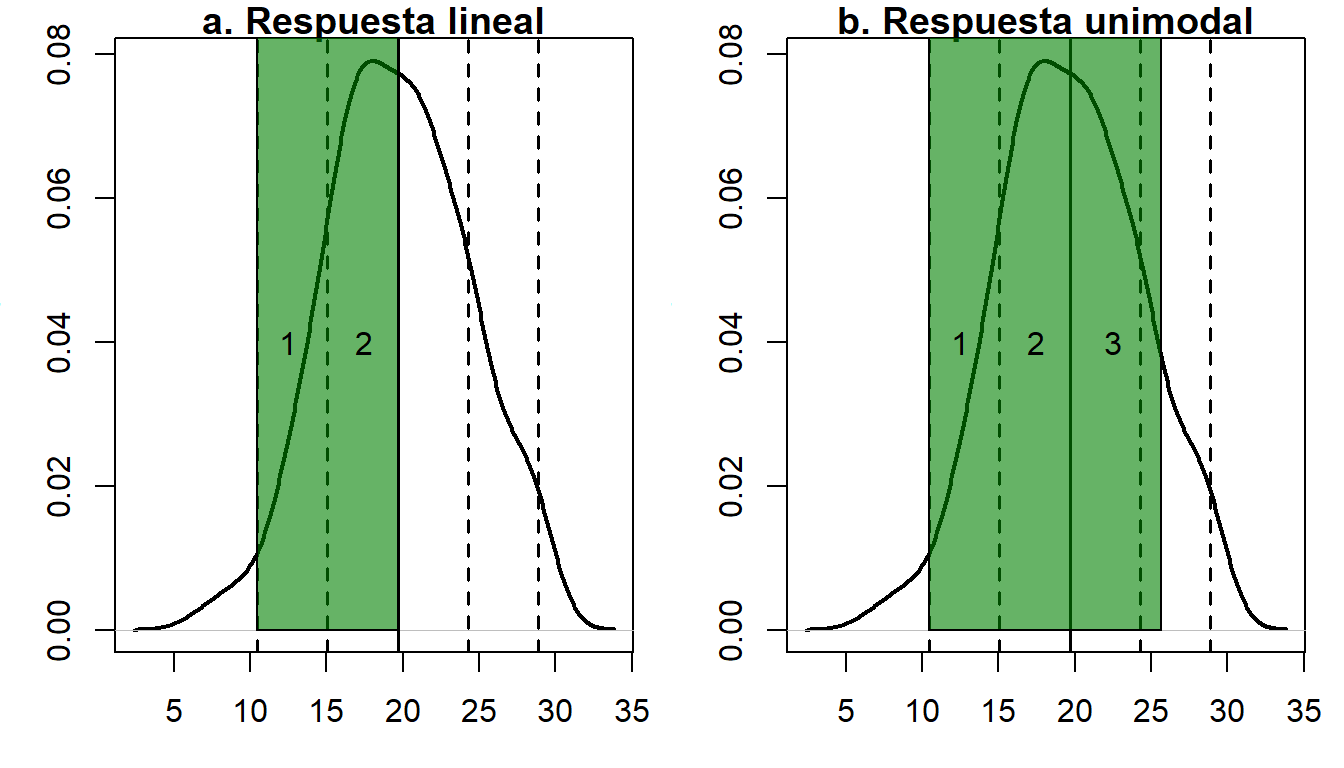
\includegraphics{AnalisisMultivarianteComunidad_files/figure-latex/resp-1.pdf}
\caption{\label{fig:resp}Definición del tipo de respuesta de la ordenación.
El área sombreada en verde y los números marcan la cantidad de
desviaciones y por lo tanto el tipo de respuesta esperado}
\end{figure}

Una vez que sabemos que tipo de respuesta tiene nuestros datos podemos
decidir el tipo de ordenación, puesto que para cada una de estas
respuestas cabe un análisis de ordenación, más adelante propondremos los
análisis de ordenación constreñida y no constreñida para cada tipo de
respuesta.

La función \emph{decorana} del paquete \textbf{vegan} nos permite
evaluar la longitud del gradiente (cantidad de desviaciones estándar).
El uso de la función \emph{decorana} necesitamos una matriz de datos con
los casos en las filas y las especies en las columnas.

\begin{Shaded}
\begin{Highlighting}[]
\KeywordTok{library}\NormalTok{(vegan)}

\CommentTok{#Cargamos los datos de Dune para usar como ejemplo}
\KeywordTok{data}\NormalTok{(dune)}

\CommentTok{#Realizamos la ordenación}
\NormalTok{ord.dca <-}\StringTok{ }\KeywordTok{decorana}\NormalTok{(dune)}

\CommentTok{#vemos el resultado de la ordenación}
\NormalTok{ord.dca}
\end{Highlighting}
\end{Shaded}

\begin{verbatim}
## 
## Call:
## decorana(veg = dune) 
## 
## Detrended correspondence analysis with 26 segments.
## Rescaling of axes with 4 iterations.
## 
##                   DCA1   DCA2    DCA3    DCA4
## Eigenvalues     0.5117 0.3036 0.12125 0.14267
## Decorana values 0.5360 0.2869 0.08136 0.04814
## Axis lengths    3.7004 3.1166 1.30055 1.47888
\end{verbatim}

Como vemos cuando ejecutamos el objeto de salida de la ordenación nos
brinda alguna información, por ahora el que nos interesa es ver las
unidades de desviación del eje 1 (DCA1). La longitud de este primer eje
(axis lengths), muestra la cantidad de desviaciones, en el ejemplo de
Dune, el eje DCA1 tiene una longitud de 3.7 unidades de desviación, con
lo cual asumimos una respuesta unimodal. Al conocer el tipo de respuesta
ya podemos decidir el tipo de ordenación (ver Tabla
\ref{tab:ordenacion}.

Algunas veces nuestros datos tienen restricciones sobre el tipo de
distancias que se pueden usar para la ordenación. Por ejemplo, en los
datos con muchos ceros no deberíamos utilizar una medida de distancia
Euclidiana, deberíamos trabajar con distancia de Bray-Curtis (Ver
ejercicio de
\href{https://ciespinosa.github.io/Similitud/index.html}{Similitud}. De
esta forma, es posible que el tipo de distancia que hemos decidido usar
defina el tipo de ordenación. En el caso del ejemplo, deberíamos usar el
Escalado Multidimensional (Multidimensional Scaling).

\textbf{2. Transformación y estandarización de los datos}

Lo siguiente que debemos decidir es si es necesario transformar o
estandarizar los datos (Ver ejercicio de
\href{https://ciespinosa.github.io/Similitud/index.html}{Similitud}).
Muchos autores aconsejan que en medida de lo posible los datos no
deberían ser transformados, sin embargo, si los datos son muy distintos
es necesario realizar la transformación. Si revisan los datos de Dune
verán que no existen diferencias importantes entre las abundancias de
cada especie, por tanto, no se requiere hacer una transformación.

\begin{quote}
Recuerden, para transformar los datos definimos la variación entre
variables. En variables con más de tres magnitudes de diferencia usamos
logaritmo y con dos magnitudes de diferencia usamos raíz cuadrada.
\end{quote}

Aunque no es necesario transformar, vamos hacer el ejercicio para
entender cómo funciona este proceso. Usaremos la función
\texttt{decostand} del paquete vegan, que se puede utilizar para la
estandarización y para la transformación.

\begin{Shaded}
\begin{Highlighting}[]
\NormalTok{dsRaiz <-}\StringTok{ }\KeywordTok{decostand}\NormalTok{(dune, }\StringTok{"standardize"}\NormalTok{, }\StringTok{"hellinger"}\NormalTok{) }
\CommentTok{#Estandarizado y transformado raíz cuadrada (hellinger)}

\NormalTok{dslog <-}\StringTok{ }\KeywordTok{decostand}\NormalTok{(dune, }\StringTok{"standardize"}\NormalTok{, }\StringTok{"log"}\NormalTok{) }
\CommentTok{#Estandarizado y transformado logaritmo (log)}

\NormalTok{dsSta <-}\StringTok{ }\KeywordTok{decostand}\NormalTok{(dune, }\StringTok{"standardize"}\NormalTok{)}
\end{Highlighting}
\end{Shaded}

Ahora que sabemos que tipo de ordenación debería realizar y mis datos
estan listos para trabajar podemos iniciar los análisis de ordenación.

\section{Ordenación indirecta o no
constreñida}\label{ordenacion-indirecta-o-no-constrenida}

Las diferentes técnicas de ordenación, a excepción de los NMDS, se basan
en la extracción de eigenvectors asociados con la matriz de datos. Los
diferentes métodos de ordenación se pueden clasificar según la distancia
preservada entre sitios y el tipo de variables que se usan.

Los métodos de ordenación como lo habíamos comentado intentan obtener
información sobre la heterogeneidad que tienen los datos. En términos
sencillos la ordenación genera una nube de puntos basado en todas las
variables (especies) que tiene nuestra comunidad, tendríamos un espacio
multidimensional. Normalmente, esa nube de puntos será más alargada en
ciertas direcciones y más aplanada en otras direcciones. La dirección
donde la nube de puntos es más aplanada se corresponde con la dirección
de mayor variabilidad de nuestros datos, donde el gradiente es más
claro. Este es el primer eje de ordenación que se deberá extraer. A
partir de aquí se buscarán otras direcciones que vayan en forma
decreciente la cantidad de variación explicada (menos alargada). Cada
eje extraído es ortogonal a los otros ejes, eso quiere decir que son
linearmente independientes y no correlacionados.

Cuando en los datos hay estructuras claras (gradientes o grupos) y el
método ha sido eficiente para extraerlas, entonces los primeros ejes
contienen la mayor parte de la información útil, es decir, han extraído
la mayor parte de la varianza de los datos. En ese caso, las distancias
entre sitios en la proyección en un espacio reducido (con mayor
frecuencia bidimensional) son relativamente similares a las distancias
entre objetos en el espacio multidimensional.

Como lo comentamos anteriormente el decidir que ordenación usar depende
del tipo de respuesta que tienen los datos y de la distancia que se
utilizará. De esta forma, si los datos muestran una respuesta lineal se
puede usar un análisis de componentes principales (PCA), mientras que si
es unimodal podemos ajustar un análisis de correspondiente (CA) o
análisis de correspondencia sin tendencia (DCA) (Tabla
\ref{tab:ordenacion})

\begin{table}[t]

\caption{\label{tab:ordenacion}Relación entre el tipo de variable y el método de ordenación no constreñida a utilizar}
\centering
\begin{tabular}{ll}
\toprule
Medidas.de.Similitud & Tipo.de.Ordenación\\
\midrule
Respuesta lineal & PCA\\
Respuesta Unimodal & CA/DCA\\
Bray-Curtis & PcoA/mMDS/nmMDS\\
\bottomrule
\end{tabular}
\end{table}

\subsection{Métodos de ordenación.}\label{metodos-de-ordenacion.}

\textbf{\emph{1. Principal Component Analysis (PCA)}}

Esta técnica de ordenación es sencilla de interpretar, las distancias
entre las muestras son interpretadas directamente como distancias
euclidianas. Este método de ordenación es ampliamente usado con datos
ambientales, donde el valor de cero es informativo, aunque se puede usar
en datos biológicos previo una transformación. El PCA al usar distancias
euclidianas es fuertemente afectado por ceros, y detecta relaciones
lineares de los datos.

Además de las limitantes de los dobles ceros, otro inconveniente que
puede tener esta ordenación, es que la proyección de las distancias
euclidias en un plano puede distorsionar algunas distancias en otros
planos.

Los gráficos de dispersión de la ordenación PCA, los objetos (las
comunidades) se representan como puntos y las variables se muestran como
flechas.

Ahora vamos hacer un ejercicio rápido y ajustar un PCA a datos de
arrestos en Estados Unidos. Estos datos que se encuentran en el paquete
base de R contiene el porcentaje de asaltos (Assault), asesinatos
(Murder) y secuestros (Rape) por cada 100,000 habitantes para cada uno
de los 50 estados de USA (1973). Además, también incluye el porcentaje
de la población de cada estado que vive en zonas rurales (UrbanPoP).

\begin{Shaded}
\begin{Highlighting}[]
\KeywordTok{library}\NormalTok{(vegan)}
\KeywordTok{data}\NormalTok{(}\StringTok{"USArrests"}\NormalTok{)}
\KeywordTok{head}\NormalTok{(USArrests, }\DecValTok{4}\NormalTok{)}
\end{Highlighting}
\end{Shaded}

\begin{verbatim}
##          Murder Assault UrbanPop Rape
## Alabama    13.2     236       58 21.2
## Alaska     10.0     263       48 44.5
## Arizona     8.1     294       80 31.0
## Arkansas    8.8     190       50 19.5
\end{verbatim}

\begin{Shaded}
\begin{Highlighting}[]
\CommentTok{#usaremos la función rda para ajustar un pca}
\NormalTok{pca.Arr <-}\StringTok{ }\KeywordTok{rda}\NormalTok{(USArrests, }\DataTypeTok{scale =} \OtherTok{TRUE}\NormalTok{)}

\CommentTok{#el argumento scale = TRUE nos permite estandarizar los datos }
\CommentTok{#los arrestos como vemos son mucho más altos que las otras variables}

\CommentTok{#Vemos el resultado del ajuste}
\NormalTok{pca.summ <-}\StringTok{ }\KeywordTok{summary}\NormalTok{(pca.Arr)}

\CommentTok{#Eigenvalues}
\CommentTok{#para obtener los eignvalues le pedimos que del objeto que contiene el resumen del}
\CommentTok{#análisis (pca.summ) el elemento cont }
\NormalTok{pca.summ$cont}
\end{Highlighting}
\end{Shaded}

\begin{verbatim}
## $importance
## Importance of components:
##                          PC1    PC2     PC3     PC4
## Eigenvalue            2.4802 0.9898 0.35656 0.17343
## Proportion Explained  0.6201 0.2474 0.08914 0.04336
## Cumulative Proportion 0.6201 0.8675 0.95664 1.00000
\end{verbatim}

Los \emph{eigenvalores} son medidas de la importancia (varianza) de los
ejes. Pueden expresarse como proporciones explicadas, o proporciones de
variación explicadas, dividiéndolas por la inercia total. En el caso del
ejemplo vemos que el componente 1 (PC1) explica el 62\% de la varianza
de nuestros datos, y el segundo componente (PC2) el 24\% en conjunto
estos dos componentes explican el 86\% de la variación de los datos.

\begin{Shaded}
\begin{Highlighting}[]
\CommentTok{#puntuación de las especies }
\NormalTok{pca.summ$species}
\end{Highlighting}
\end{Shaded}

\begin{verbatim}
##                 PC1        PC2        PC3         PC4
## Murder   -1.5789353  0.7783309 -0.3812000  0.50581692
## Assault  -1.7182500  0.3498845 -0.2995557 -0.57919282
## UrbanPop -0.8196414 -1.6244933 -0.4222914  0.10430487
## Rape     -1.6011289 -0.3114185  0.9135612  0.06935934
\end{verbatim}

La puntuación de las especies nos muestra cómo se asocia el primer
componente a esa variable y el peso de esa variable. De esta forma, en
el ejemplo, en el primer componente las variables Assault, Murder y Rape
son aproximadamente iguales entre ellas y bastante superiores al
asignado a UrbanPoP y tienen una asociación negativa. En el caso del
componente dos UrbanPop tiene un peso más importante en ese eje y su
relación es negativa. Cuando usamos \emph{vegan} para ajustar una
ordenación las variables siempre serán mostradas como especies.

\begin{Shaded}
\begin{Highlighting}[]
\CommentTok{#Sitios}
\CommentTok{#Usamos la función head para que se despliegue únicamente los 6 primeros sitios}
\KeywordTok{head}\NormalTok{(pca.summ$sites)}
\end{Highlighting}
\end{Shaded}

\begin{verbatim}
##                    PC1        PC2         PC3         PC4
## Alabama    -0.33114461  0.6028277 -0.39369198  0.19855667
## Alaska     -0.65523534  0.5708197  1.80776363 -0.55727431
## Arizona    -0.59241305 -0.3967588  0.04854442 -1.06052940
## Arkansas    0.04751642  0.5955965  0.10153030 -0.23228377
## California -0.84804316 -0.8206544  0.53041541 -0.43454867
## Colorado   -0.50888462 -0.5252599  0.97034832  0.00186132
\end{verbatim}

Sitios se refiere al valor que recibe cada uno de los sitios
(observaciones) en cada uno de los componentes, en un gráfico de doble
entrada serían las coordenadas.

Finalmente, cuando queremos mostrar nuestra ordenación en un biplot o
gráfico de dispersión, la forma en que se muestran los resultados puede
estar definidos de dos formas distintas. Scaling 1 es usado normalmente
cuando nos interesa ver las diferencias entre los sitios. Mientras que
scaling 2 es usado si lo que nos interesa es evaluar la relación entre
las variables. Veamos la diferencia en la representación gráfica.

\begin{Shaded}
\begin{Highlighting}[]
\KeywordTok{par}\NormalTok{(}\DataTypeTok{mfcol=}\KeywordTok{c}\NormalTok{(}\DecValTok{1}\NormalTok{,}\DecValTok{2}\NormalTok{))}

\KeywordTok{biplot}\NormalTok{(pca.Arr, }\DataTypeTok{scaling=}\DecValTok{1}\NormalTok{, }\DataTypeTok{main =} \StringTok{"Scaling 1"}\NormalTok{)}
\KeywordTok{biplot}\NormalTok{(pca.Arr, }\DataTypeTok{scaling=}\DecValTok{2}\NormalTok{, }\DataTypeTok{main =} \StringTok{"Scaling 2"}\NormalTok{)}
\end{Highlighting}
\end{Shaded}

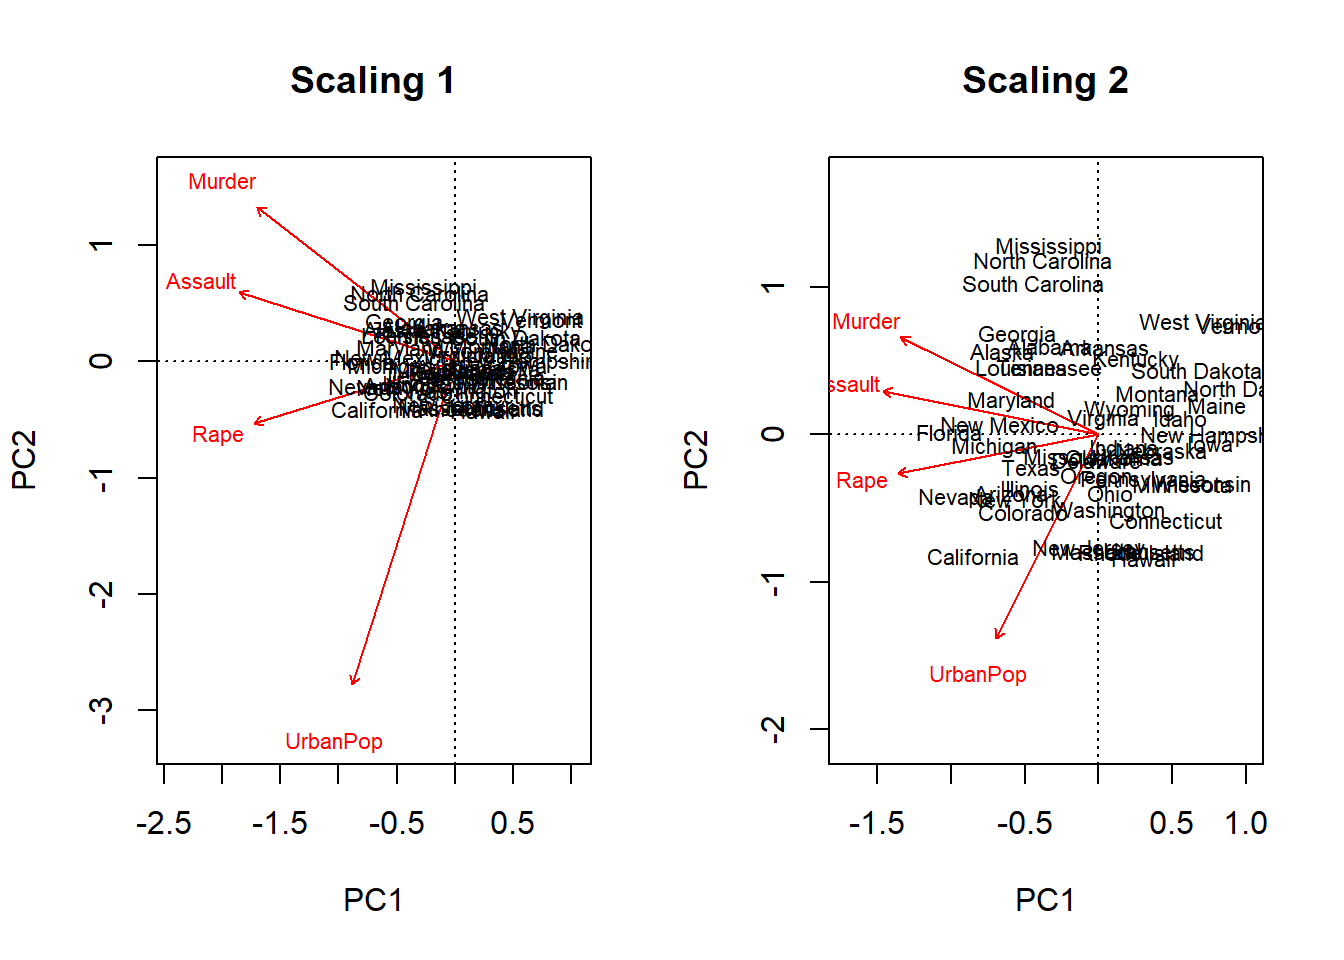
\includegraphics{AnalisisMultivarianteComunidad_files/figure-latex/unnamed-chunk-13-1.pdf}

\textbf{\emph{2. Principal Coordinates Análisis (PCoA)}}

PCoA, conocido también como escalado métrico multidimensional (MDS) es
conceptualmente similar a PCA y análisis de correspondencia (CA) que
preservan distancias Eudlicean y chi-cuadrado entre objetos,
respectivamente, la diferencia con estos métodos de ordenación es que el
PCoA puede preservar las distancias generadas a partir de cualquier
medida de similitud o disimilitud permitiendo un manejo más flexible de
datos ecológicos complejos. PCA se usa comúnmente para similitudes y
PCoA para diferencias.

Una ventaja importante es que el PCoA permite manejar matrices de
disimilitud calculadas a partir de variables cuantitativas,
semicuantitativas, cualitativas y mixtas. En este caso la elección de la
medida de similitud o disimilitud es crítica y debe ser adecuada para
los datos con los que se está trabajando.

Aunque, este método presenta varias ventajas hay que recordad que el
PCoA representa en el plano los componentes euclidianos de la matriz,
incluso si la matriz contiene distancias no euclidianas.

Usaremos el paquete \textbf{ape} para implementar el PCoA y la función
\emph{pcoa} que computa la ordenación, para esto necesitamos una matriz
de distancias o similitudes como entrada, usaremos el paquete
\textbf{cluster} y la función \emph{daisy} para calcular la distancia de
gower.

\begin{Shaded}
\begin{Highlighting}[]
\CommentTok{#cargamos datos de ejemplo}
\KeywordTok{library}\NormalTok{(vegan)}
\KeywordTok{data}\NormalTok{(}\StringTok{"dune.env"}\NormalTok{)}

\CommentTok{#calculamos la distancia de gower con datos mixtos}
\CommentTok{#variables numéricas y categóricas}
\KeywordTok{library}\NormalTok{(cluster)}
\NormalTok{disGow <-}\StringTok{ }\KeywordTok{daisy}\NormalTok{(dune.env, }\StringTok{"gower"}\NormalTok{)}

\CommentTok{#realizamos la ordenación y graficamos}
\KeywordTok{library}\NormalTok{(ape)}
\NormalTok{pcoaDun <-}\StringTok{ }\KeywordTok{pcoa}\NormalTok{(disGow)}

\CommentTok{#vemos los eigenvalores}
\KeywordTok{head}\NormalTok{(pcoaDun$values)}
\end{Highlighting}
\end{Shaded}

\begin{verbatim}
##   Eigenvalues Relative_eig Rel_corr_eig Broken_stick Cum_corr_eig
## 1  1.19219411   0.48682576   0.23125629   0.19417267    0.2312563
## 2  0.82108733   0.33528639   0.16891396   0.13861712    0.4001702
## 3  0.43337263   0.17696527   0.10378167   0.11083934    0.5039519
## 4  0.29088374   0.11878074   0.07984492   0.09232082    0.5837968
## 5  0.16285907   0.06650258   0.05833802   0.07843193    0.6421349
## 6  0.09522366   0.03888405   0.04697593   0.06732082    0.6891108
##   Cumul_br_stick
## 1      0.1941727
## 2      0.3327898
## 3      0.4436291
## 4      0.5359499
## 5      0.6143819
## 6      0.6817027
\end{verbatim}

\begin{Shaded}
\begin{Highlighting}[]
\CommentTok{#Estos nos muestran la importancia de cada variable para cada sitio}

\CommentTok{#Vemos los eigenvectores}
\KeywordTok{head}\NormalTok{(pcoaDun$vectors)}
\end{Highlighting}
\end{Shaded}

\begin{verbatim}
##       Axis.1       Axis.2      Axis.3       Axis.4       Axis.5
## 1 -0.3443117 -0.006165232 -0.17924745  0.064288860  0.074076828
## 2 -0.1739767 -0.186573785 -0.01909423  0.139208775 -0.031395356
## 3 -0.2427457  0.082399005 -0.19564033  0.005128101 -0.001429953
## 4 -0.2431447  0.080725620 -0.19479484  0.004387051 -0.009284373
## 5 -0.1023988 -0.237047606  0.07382832 -0.197239144  0.090734919
## 6 -0.1898342 -0.136476269  0.09302420 -0.081997169  0.120775554
##        Axis.6      Axis.7      Axis.8       Axis.9
## 1 -0.05466493  0.07969362 -0.01353679  0.003088923
## 2  0.14465676  0.01811985 -0.04251420 -0.001681605
## 3 -0.06254740 -0.06382868 -0.01038631 -0.007311375
## 4 -0.06626271 -0.06479374 -0.01775386  0.005158402
## 5  0.03100643  0.06066075  0.04952928 -0.005193289
## 6  0.08378295 -0.06217703 -0.02778954  0.002705063
\end{verbatim}

\begin{Shaded}
\begin{Highlighting}[]
\CommentTok{#son los vectores que se usan para la ordenación }
\end{Highlighting}
\end{Shaded}

Muy bien ahora podemos graficar los datos y ver como se organizan en el
espacio.

\begin{Shaded}
\begin{Highlighting}[]
\KeywordTok{plot}\NormalTok{(pcoaDun$vectors[,}\DecValTok{1}\NormalTok{], pcoaDun$vectors[,}\DecValTok{2}\NormalTok{], }\DataTypeTok{type =} \StringTok{"n"}\NormalTok{, }\DataTypeTok{xlab =} \StringTok{"PCoA1"}\NormalTok{, }\DataTypeTok{ylab =} \StringTok{"PCoA2"}\NormalTok{,}
 \DataTypeTok{axes =} \OtherTok{TRUE}\NormalTok{, }\DataTypeTok{main =} \StringTok{"PCoA dune.env data"}\NormalTok{)}

\KeywordTok{text}\NormalTok{(pcoaDun$vectors[,}\DecValTok{1}\NormalTok{], pcoaDun$vectors[,}\DecValTok{2}\NormalTok{], }\KeywordTok{labels}\NormalTok{(disGow), }
 \DataTypeTok{cex =} \FloatTok{0.9}\NormalTok{, }\DataTypeTok{xpd =} \OtherTok{TRUE}\NormalTok{)}
\end{Highlighting}
\end{Shaded}

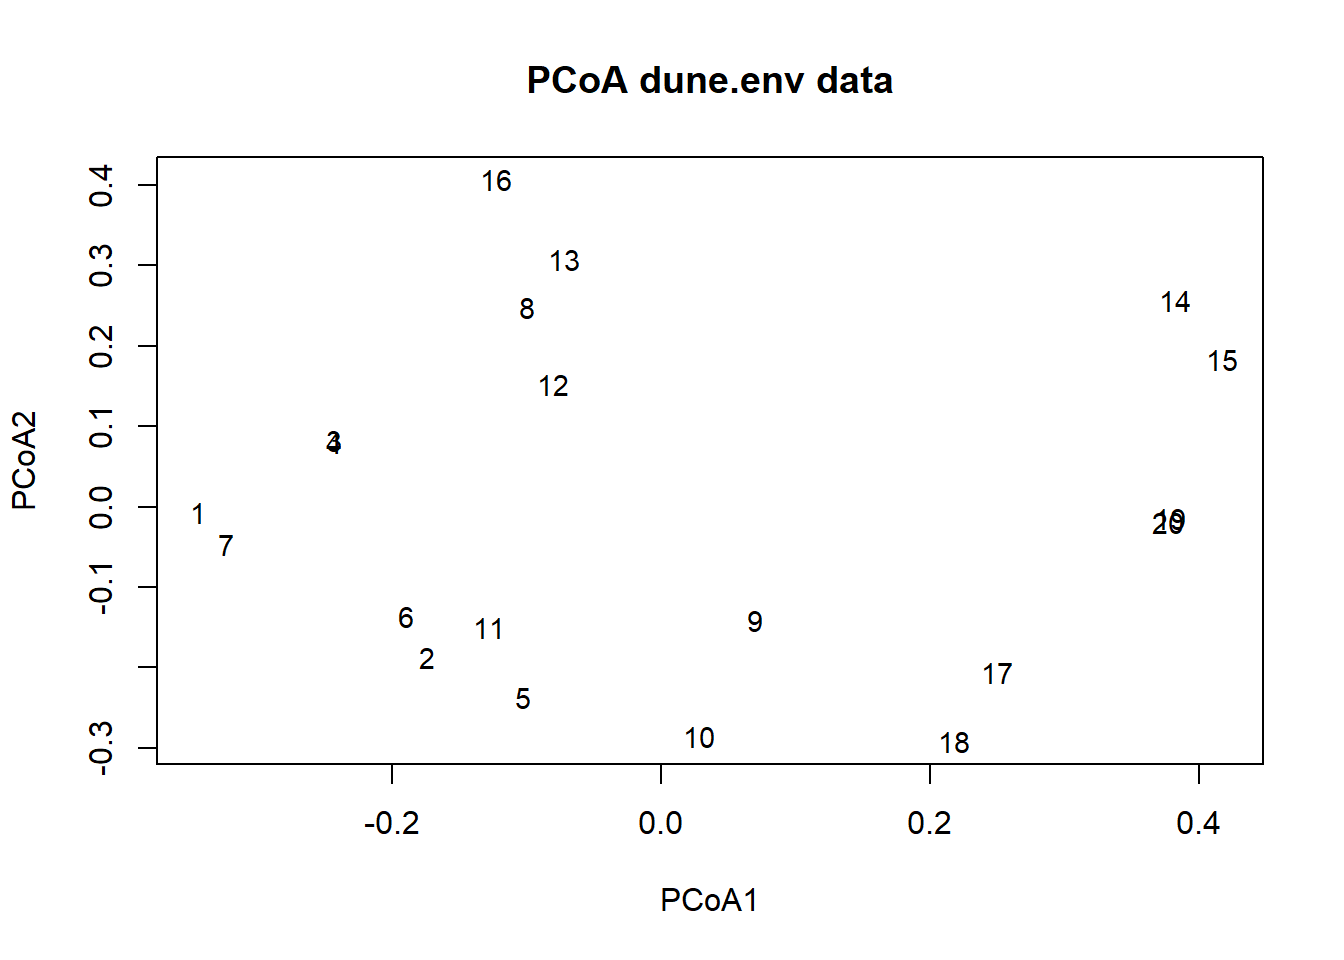
\includegraphics{AnalisisMultivarianteComunidad_files/figure-latex/unnamed-chunk-15-1.pdf}

\textbf{\emph{3. Correspondence Analysis (CA)}}

Implícitamente se generan distancias de Chi-cuadrado entre las muestras
por lo que no es afectado por matrices con dobles ceros. Se basa en un
modelo de respuesta unimodal de las especies a los gradientes
ambientales subyacentes. Uno de los principales problemas de este
análisis es que la ordenación genera un ``Efecto arco'' causado por la
respuesta unimodal de la abundancia de especies a un gradiente
ambiental.

Este análisis es implementado dentro del paquete \textbf{vegan}, para
ajustar un CA usamos la función \emph{cca}

\begin{Shaded}
\begin{Highlighting}[]
\KeywordTok{data}\NormalTok{(dune)}

\CommentTok{#ajustamos el ca}
\NormalTok{ca.dune <-}\StringTok{ }\KeywordTok{cca}\NormalTok{(dune)}

\CommentTok{#extraemos los datos}
\NormalTok{caSum <-}\StringTok{ }\KeywordTok{summary}\NormalTok{(ca.dune)}

\CommentTok{#Eigenvalores}
\NormalTok{caSum$cont}
\end{Highlighting}
\end{Shaded}

\begin{verbatim}
## $importance
## Importance of components:
##                          CA1    CA2    CA3     CA4     CA5     CA6     CA7
## Eigenvalue            0.5360 0.4001 0.2598 0.17598 0.14476 0.10791 0.09247
## Proportion Explained  0.2534 0.1892 0.1228 0.08319 0.06844 0.05102 0.04372
## Cumulative Proportion 0.2534 0.4426 0.5654 0.64858 0.71702 0.76804 0.81175
##                           CA8     CA9    CA10    CA11    CA12    CA13
## Eigenvalue            0.08091 0.07332 0.05630 0.04826 0.04125 0.03523
## Proportion Explained  0.03825 0.03466 0.02661 0.02282 0.01950 0.01665
## Cumulative Proportion 0.85000 0.88467 0.91128 0.93410 0.95360 0.97025
##                           CA14     CA15     CA16     CA17     CA18
## Eigenvalue            0.020529 0.014911 0.009074 0.007938 0.007002
## Proportion Explained  0.009705 0.007049 0.004290 0.003753 0.003310
## Cumulative Proportion 0.979955 0.987004 0.991293 0.995046 0.998356
##                           CA19
## Eigenvalue            0.003477
## Proportion Explained  0.001644
## Cumulative Proportion 1.000000
\end{verbatim}

\begin{Shaded}
\begin{Highlighting}[]
\CommentTok{#el primer componente explica el 25% de la variación}

\CommentTok{#Ahora graficamos}
\KeywordTok{par}\NormalTok{(}\DataTypeTok{mfcol=}\KeywordTok{c}\NormalTok{(}\DecValTok{1}\NormalTok{,}\DecValTok{2}\NormalTok{))}
\KeywordTok{plot}\NormalTok{(ca.dune, }\DataTypeTok{scaling =} \DecValTok{1}\NormalTok{, }\DataTypeTok{main=}\StringTok{"CA scaling 1"}\NormalTok{)}
\KeywordTok{plot}\NormalTok{(ca.dune, }\DataTypeTok{scaling =} \DecValTok{2}\NormalTok{, }\DataTypeTok{main=}\StringTok{"CA scaling 2"}\NormalTok{)}
\end{Highlighting}
\end{Shaded}

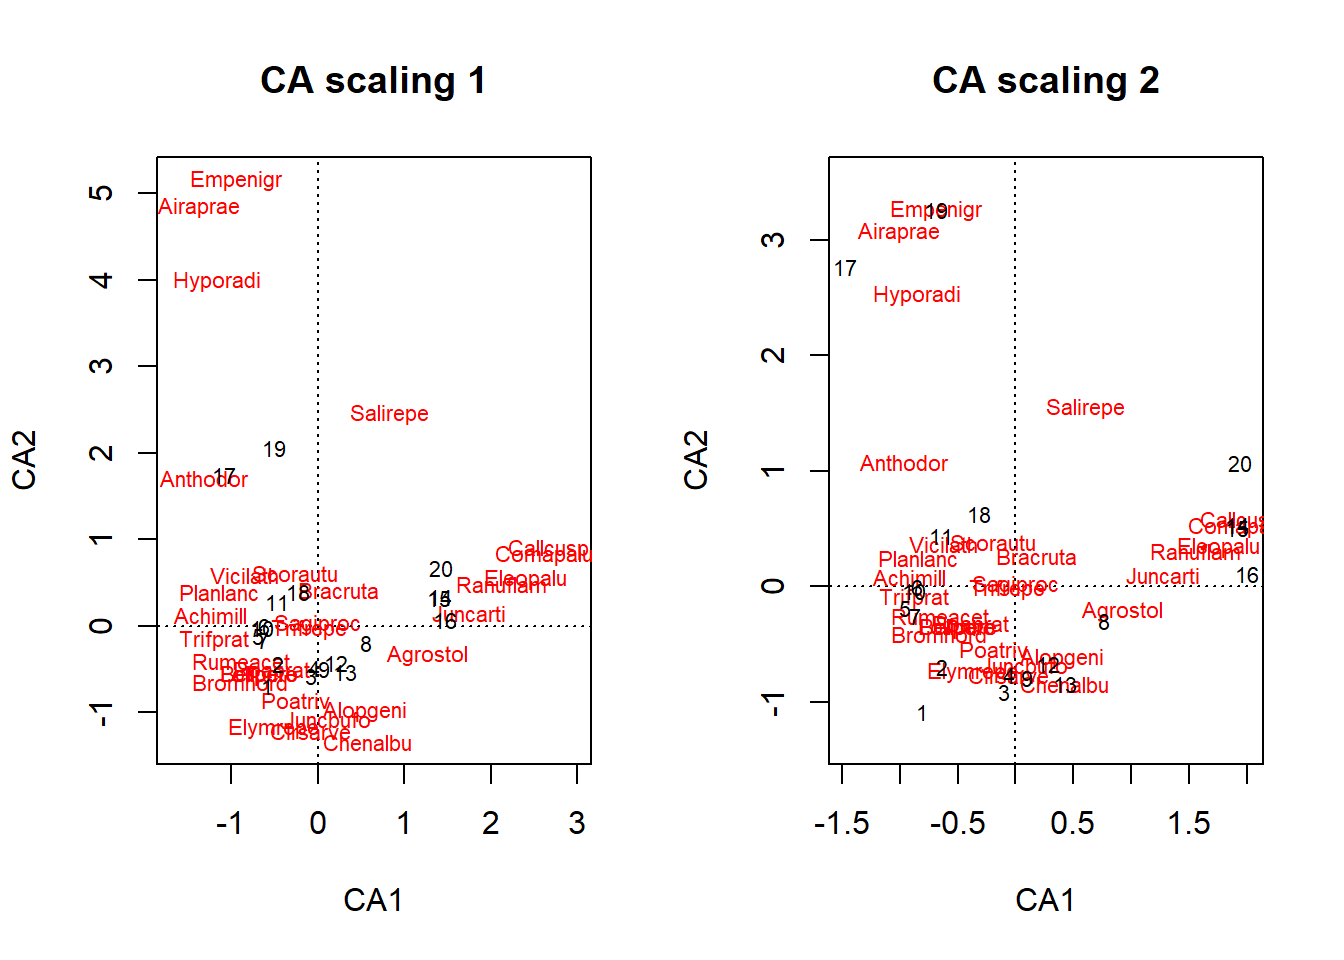
\includegraphics{AnalisisMultivarianteComunidad_files/figure-latex/unnamed-chunk-16-1.pdf}

\textbf{Recuerde:} Al igual que en el PCA usamos \emph{scaling 1} cuando
lo que nos interesa es evaluar la relación entre sitios, mientras que
\emph{scaling 2} usamos cuando nos interesa evaluar la relación entre
especies.

\textbf{\emph{4. Detrended Correspondence Analysis (DCA, DECORANA)}}

Es una extensión del CA que corrige el efecto arco. Este método realiza
una ordenación por segmentos y luego los alinea con el fin de evitar la
curvatura. Muchos autores proponen que este tipo de análisis implica una
excesiva manipulación de los datos (Pielou 1984).

Este análisis es implementado dentro del paquete \textbf{vegan}, para
ajustar un CA usamos la función \emph{dca}

\begin{Shaded}
\begin{Highlighting}[]
\CommentTok{#ajustamos el dca}
\NormalTok{dca.dune <-}\StringTok{ }\KeywordTok{decorana}\NormalTok{(dune)}
\NormalTok{dca.dune}
\end{Highlighting}
\end{Shaded}

\begin{verbatim}
## 
## Call:
## decorana(veg = dune) 
## 
## Detrended correspondence analysis with 26 segments.
## Rescaling of axes with 4 iterations.
## 
##                   DCA1   DCA2    DCA3    DCA4
## Eigenvalues     0.5117 0.3036 0.12125 0.14267
## Decorana values 0.5360 0.2869 0.08136 0.04814
## Axis lengths    3.7004 3.1166 1.30055 1.47888
\end{verbatim}

\begin{Shaded}
\begin{Highlighting}[]
\CommentTok{#Ahora graficamos}
\KeywordTok{par}\NormalTok{(}\DataTypeTok{mfcol=}\KeywordTok{c}\NormalTok{(}\DecValTok{1}\NormalTok{,}\DecValTok{2}\NormalTok{))}
\KeywordTok{plot}\NormalTok{(dca.dune)}
\end{Highlighting}
\end{Shaded}

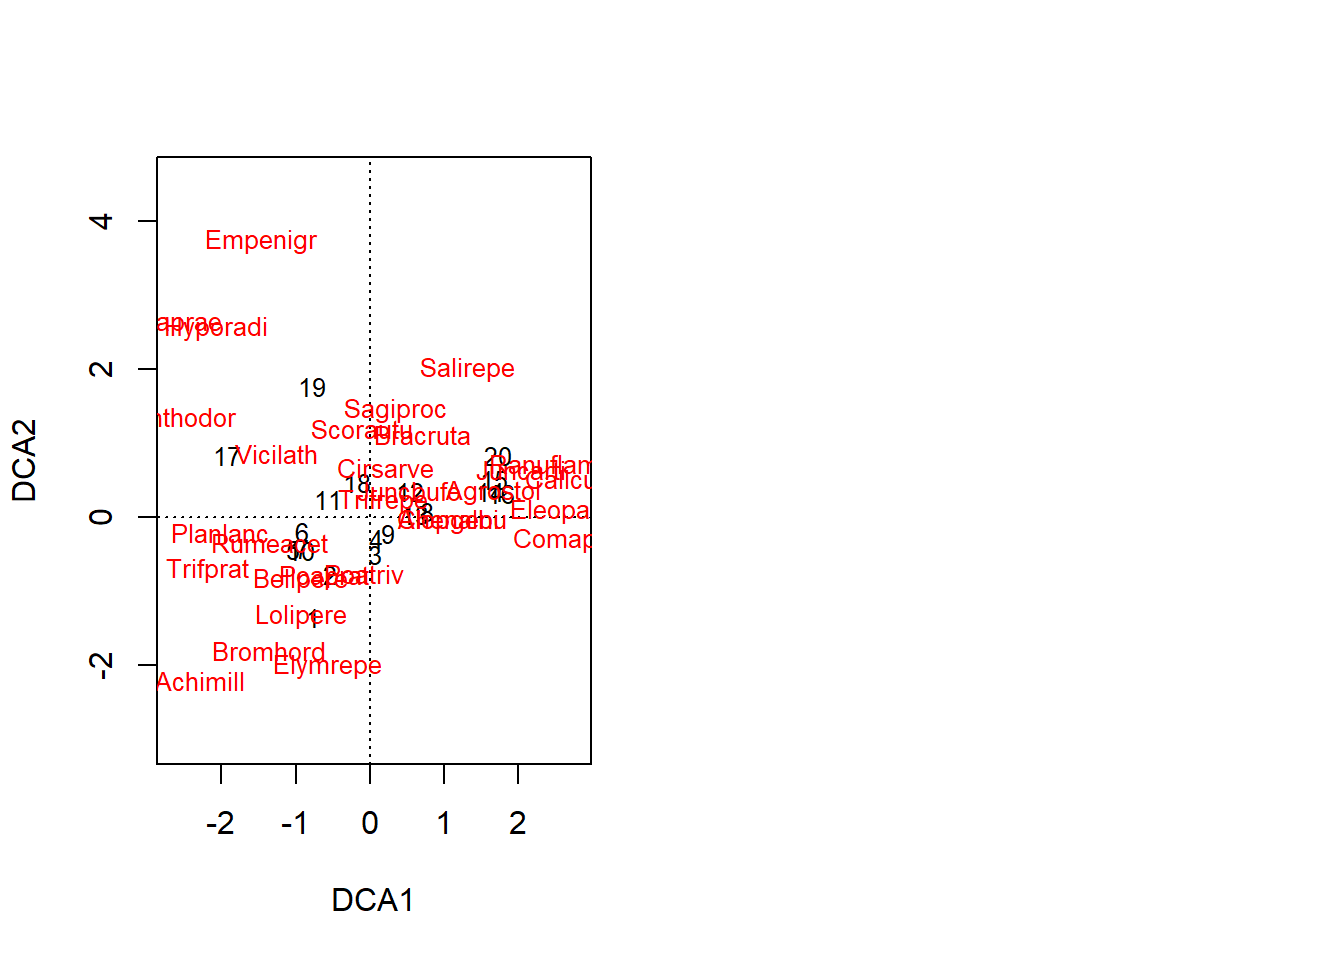
\includegraphics{AnalisisMultivarianteComunidad_files/figure-latex/unnamed-chunk-17-1.pdf}
\textbf{\emph{5. Nonmetric Multidimensional Scaling (NMDS)}}

Una de las principales características de este método es que permite
ajustar la ordenación con cualquier método de distancias. De esta forma
se pueden usar distancias que sean biológicamente relevantes. Un
problema de este método es que la ordenación de las muestras utiliza el
orden relativo de las distancias entre muestras y no los valores
absolutos de los coeficientes de similitud. Esto significa que si la
muestra 1 es más parecida a la 2 que a la 3 entonces se localizará más
cercana a la muestra 2 que a la 3, sin embargo, esa diferencias entre
distancias no necesariamente tendrá la dimensión exacta. Por eso la
representación gráfica del nMDS sufre menos distorsiones respecto a las
distancias reales.

\begin{Shaded}
\begin{Highlighting}[]
\NormalTok{nmds.dune <-}\StringTok{ }\KeywordTok{metaMDS}\NormalTok{(dune,}\DataTypeTok{distance=}\StringTok{"bray"}\NormalTok{, }\DataTypeTok{k=}\DecValTok{2}\NormalTok{, }\DataTypeTok{trymax=}\DecValTok{50}\NormalTok{)   }
\NormalTok{nmds.dune }
\end{Highlighting}
\end{Shaded}

A diferencia de los otros métodos que hemos visto hasta aquí el NMDS, el
stress es el que nos muestra que tan efectiva ha sido la ordenación. El
valor de estrés (stress) nos indica la cantidad de varianza que
\textbf{NO} se ajustó, mientras más bajo es el estrés mayor varianza
explica. Una regla general, aunque discutida, es que las ordenaciones
con estrés \textgreater{}0.05 proporciona una representación
\emph{excelente} en las dimensiones reducidas, \textgreater{}0.1 es
\emph{muy bueno}, \textgreater{}0.2 es \emph{bueno} con valores de
estrés \textgreater{}0.3 se dice que la ordenación proporciona una pobre
representación de la variación de los datos. En nuestro ejemplo el
estrés podría considerarse muy bueno.

\begin{Shaded}
\begin{Highlighting}[]
\CommentTok{#graficamos la ordenación}

\KeywordTok{plot}\NormalTok{(nmds.dune, }\DataTypeTok{main=}\StringTok{"NMDS de los datos de Dune"}\NormalTok{)}
\end{Highlighting}
\end{Shaded}

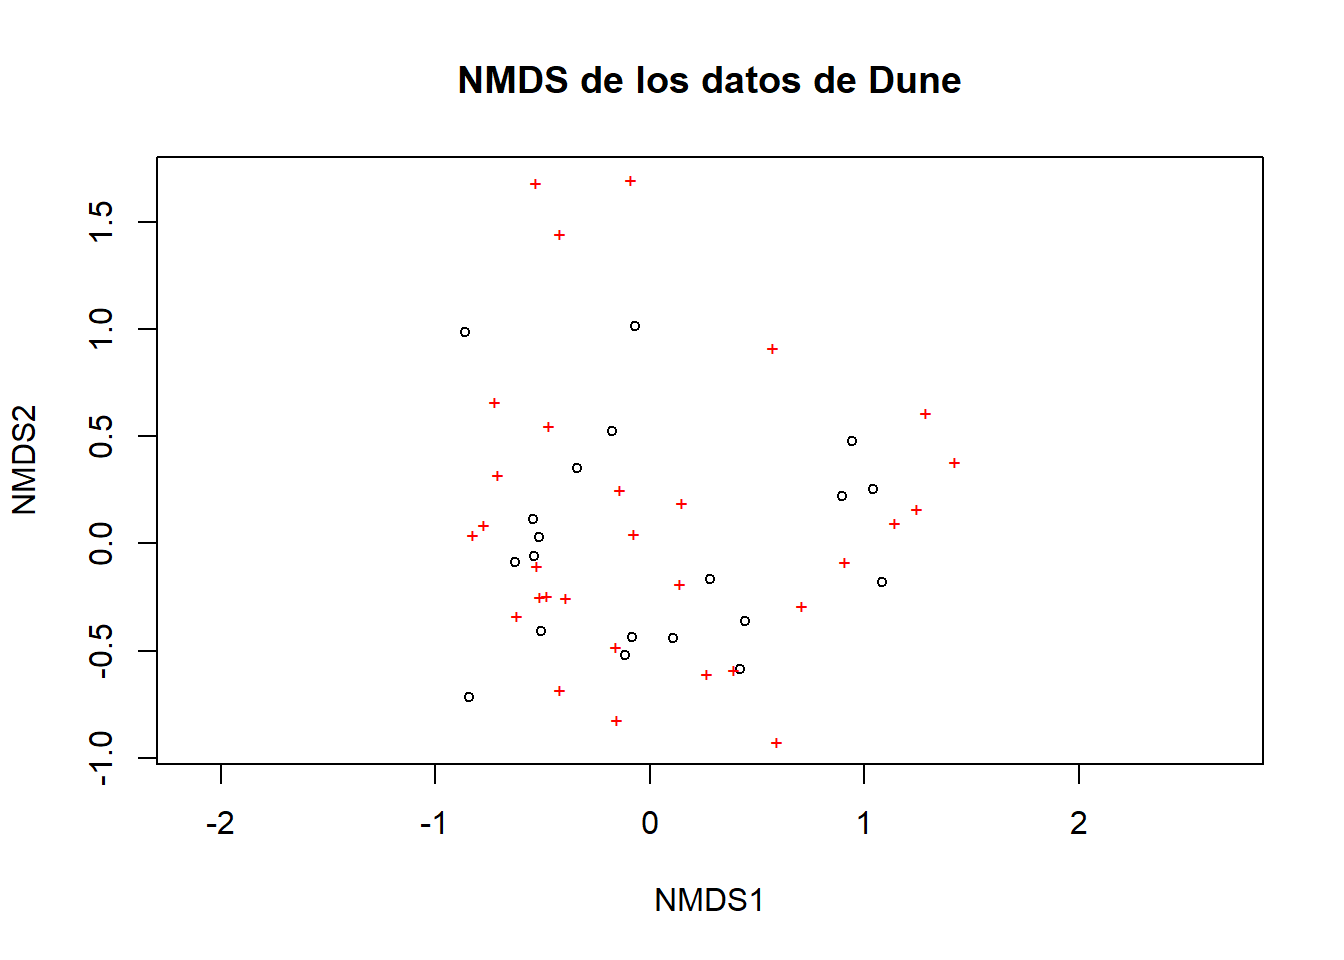
\includegraphics{AnalisisMultivarianteComunidad_files/figure-latex/unnamed-chunk-19-1.pdf}

\subsection{Graficar los resultados}\label{graficar-los-resultados}

Como hemos visto existen diferentes formas de graficar los resultados de
la ordenación. A continuación mostramos una forma de personalización del
gráfico de ordenación que se aplica a la mayor parte de ordenaciones.

\begin{Shaded}
\begin{Highlighting}[]
\KeywordTok{plot}\NormalTok{(nmds.dune, }\DataTypeTok{type=}\StringTok{"n"}\NormalTok{)  }\CommentTok{# para dibujar un plot vacío}
\KeywordTok{points}\NormalTok{(nmds.dune, }\DataTypeTok{display=}\StringTok{"sites"}\NormalTok{, }\DataTypeTok{cex=}\FloatTok{0.8}\NormalTok{, }\DataTypeTok{pch=}\DecValTok{21}\NormalTok{, }\DataTypeTok{col=}\StringTok{"black"}\NormalTok{, }\DataTypeTok{bg=}\StringTok{"yellow"}\NormalTok{)  }
\KeywordTok{text}\NormalTok{(nmds.dune, }\DataTypeTok{display=} \StringTok{"spec"}\NormalTok{, }\DataTypeTok{cex=}\FloatTok{0.5}\NormalTok{, }\DataTypeTok{col=}\StringTok{"blue"}\NormalTok{) }
\end{Highlighting}
\end{Shaded}

\begin{figure}

{\centering 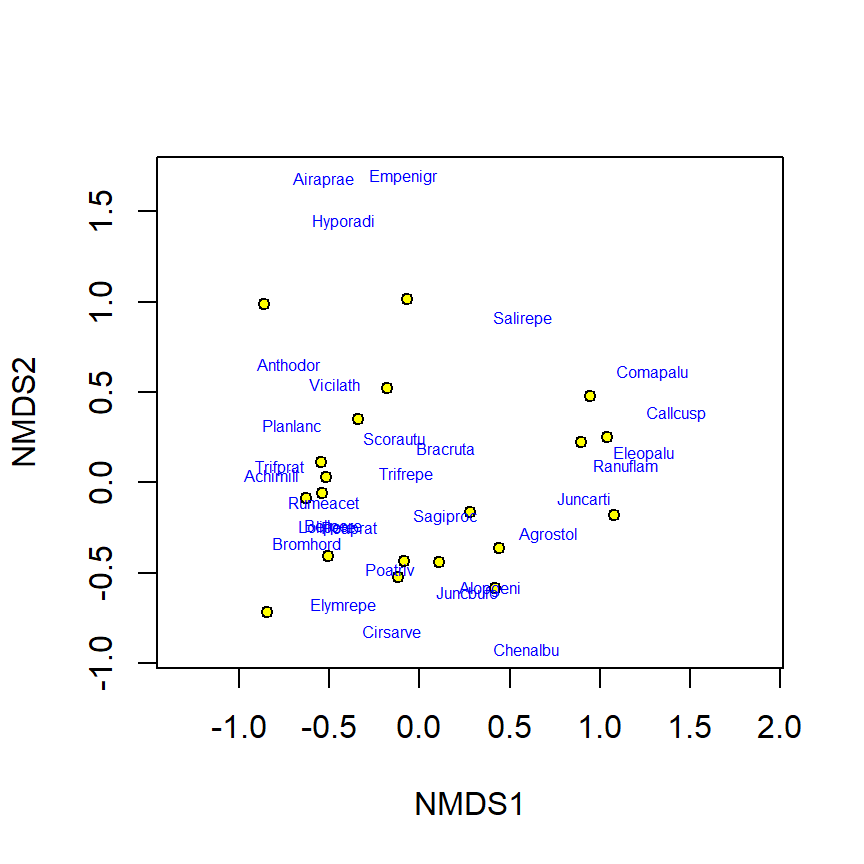
\includegraphics{AnalisisMultivarianteComunidad_files/figure-latex/plotnmds-1} 

}

\caption{Representación gráfica del NMDS}\label{fig:plotnmds}
\end{figure}

Podemos ver en la figura \ref{fig:plotnmds} que ciertas especies están
asociadas con ciertas localidades esto nos podría servir para explorar
los datos.

\subsection{Interpretación ambiental}\label{interpretacion-ambiental}

Como lo mencionamos previamente las ordenaciones indirectas no sirven
para testar hipótesis, este método nos permite organizar nuestras
variables en un espacio dimensional más reducido. Sin embargo, podríamos
usar estos ejes y relacionarlos con variables ambientales. Vamos a usar
el paquete vegan para ajustar un modelo que permita evaluar el efecto de
las variables ambientales a la ordenación.

\begin{Shaded}
\begin{Highlighting}[]
\KeywordTok{data}\NormalTok{(varechem)}
\KeywordTok{data}\NormalTok{(varespec)}
\NormalTok{vare.mds <-}\StringTok{ }\KeywordTok{metaMDS}\NormalTok{(varespec, }\DataTypeTok{trace =} \OtherTok{FALSE}\NormalTok{)}
\NormalTok{ef <-}\StringTok{ }\KeywordTok{envfit}\NormalTok{(vare.mds, varechem, }\DataTypeTok{permu =} \DecValTok{999}\NormalTok{)}
\NormalTok{ef}
\end{Highlighting}
\end{Shaded}

\begin{verbatim}
## 
## ***VECTORS
## 
##             NMDS1    NMDS2     r2 Pr(>r)    
## N        -0.05733 -0.99836 0.2536  0.049 *  
## P         0.61971  0.78483 0.1938  0.091 .  
## K         0.76644  0.64231 0.1809  0.125    
## Ca        0.68520  0.72836 0.4119  0.004 ** 
## Mg        0.63252  0.77454 0.4270  0.003 ** 
## S         0.19139  0.98151 0.1752  0.145    
## Al       -0.87161  0.49021 0.5269  0.001 ***
## Fe       -0.93601  0.35197 0.4451  0.003 ** 
## Mn        0.79874 -0.60167 0.5231  0.001 ***
## Zn        0.61754  0.78654 0.1879  0.104    
## Mo       -0.90311  0.42942 0.0609  0.518    
## Baresoil  0.92488 -0.38025 0.2508  0.063 .  
## Humdepth  0.93284 -0.36028 0.5201  0.001 ***
## pH       -0.64803  0.76162 0.2308  0.072 .  
## ---
## Signif. codes:  0 '***' 0.001 '**' 0.01 '*' 0.05 '.' 0.1 ' ' 1
## Permutation: free
## Number of permutations: 999
\end{verbatim}

Ahora podemos ver las variables que son significativas para explicar la
ordenación de los datos.

\begin{Shaded}
\begin{Highlighting}[]
\KeywordTok{plot}\NormalTok{(vare.mds, }\DataTypeTok{display =} \StringTok{"sites"}\NormalTok{)}
\KeywordTok{plot}\NormalTok{(ef, }\DataTypeTok{p.max =} \FloatTok{0.05}\NormalTok{)}
\end{Highlighting}
\end{Shaded}

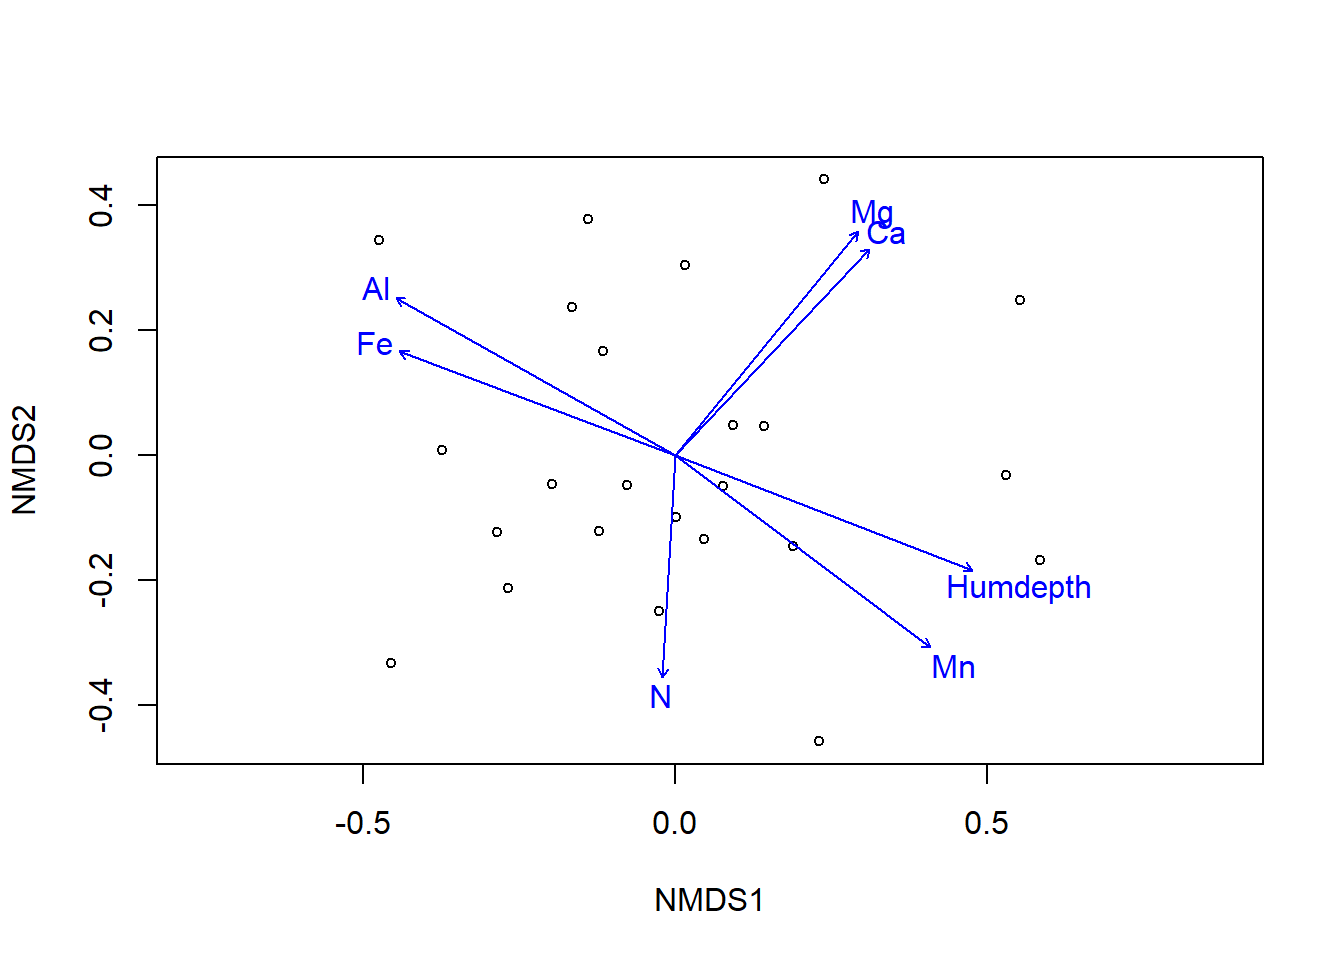
\includegraphics{AnalisisMultivarianteComunidad_files/figure-latex/unnamed-chunk-21-1.pdf}

Con variables categóricas podríamos hacer el mismo procedimiento pero
tener una gráfica de salida un poco diferente.

\begin{Shaded}
\begin{Highlighting}[]
\NormalTok{ef <-}\StringTok{ }\KeywordTok{envfit}\NormalTok{(ca.dune, dune.env, }\DataTypeTok{permutations =} \DecValTok{999}\NormalTok{)}
\NormalTok{ef}
\end{Highlighting}
\end{Shaded}

\begin{verbatim}
## 
## ***VECTORS
## 
##         CA1      CA2     r2 Pr(>r)  
## A1 0.998160 0.060614 0.3104  0.041 *
## ---
## Signif. codes:  0 '***' 0.001 '**' 0.01 '*' 0.05 '.' 0.1 ' ' 1
## Permutation: free
## Number of permutations: 999
## 
## ***FACTORS:
## 
## Centroids:
##                  CA1     CA2
## Moisture1    -0.7484 -0.1423
## Moisture2    -0.4652 -0.2156
## Moisture4     0.1827 -0.7315
## Moisture5     1.1143  0.5708
## ManagementBF -0.7258 -0.1413
## ManagementHF -0.3867 -0.2960
## ManagementNM  0.6517  1.4405
## ManagementSF  0.3376 -0.6761
## UseHayfield  -0.2861  0.6488
## UseHaypastu  -0.0735 -0.5602
## UsePasture    0.5163  0.0508
## Manure0       0.6517  1.4405
## Manure1      -0.4639 -0.1738
## Manure2      -0.5872 -0.3600
## Manure3       0.5187 -0.3172
## Manure4      -0.2059 -0.8775
## 
## Goodness of fit:
##                r2 Pr(>r)   
## Moisture   0.4113  0.005 **
## Management 0.4441  0.003 **
## Use        0.1845  0.099 . 
## Manure     0.4552  0.007 **
## ---
## Signif. codes:  0 '***' 0.001 '**' 0.01 '*' 0.05 '.' 0.1 ' ' 1
## Permutation: free
## Number of permutations: 999
\end{verbatim}

\begin{Shaded}
\begin{Highlighting}[]
\KeywordTok{plot}\NormalTok{(ca.dune, }\DataTypeTok{display =} \StringTok{"sites"}\NormalTok{, }\DataTypeTok{type =} \StringTok{"p"}\NormalTok{)}
\KeywordTok{with}\NormalTok{(dune.env, }\KeywordTok{ordiellipse}\NormalTok{(ca.dune, Management, }\DataTypeTok{kind =} \StringTok{"se"}\NormalTok{, }\DataTypeTok{conf =} \FloatTok{0.95}\NormalTok{, }\DataTypeTok{label=} \OtherTok{TRUE}\NormalTok{))}
\end{Highlighting}
\end{Shaded}

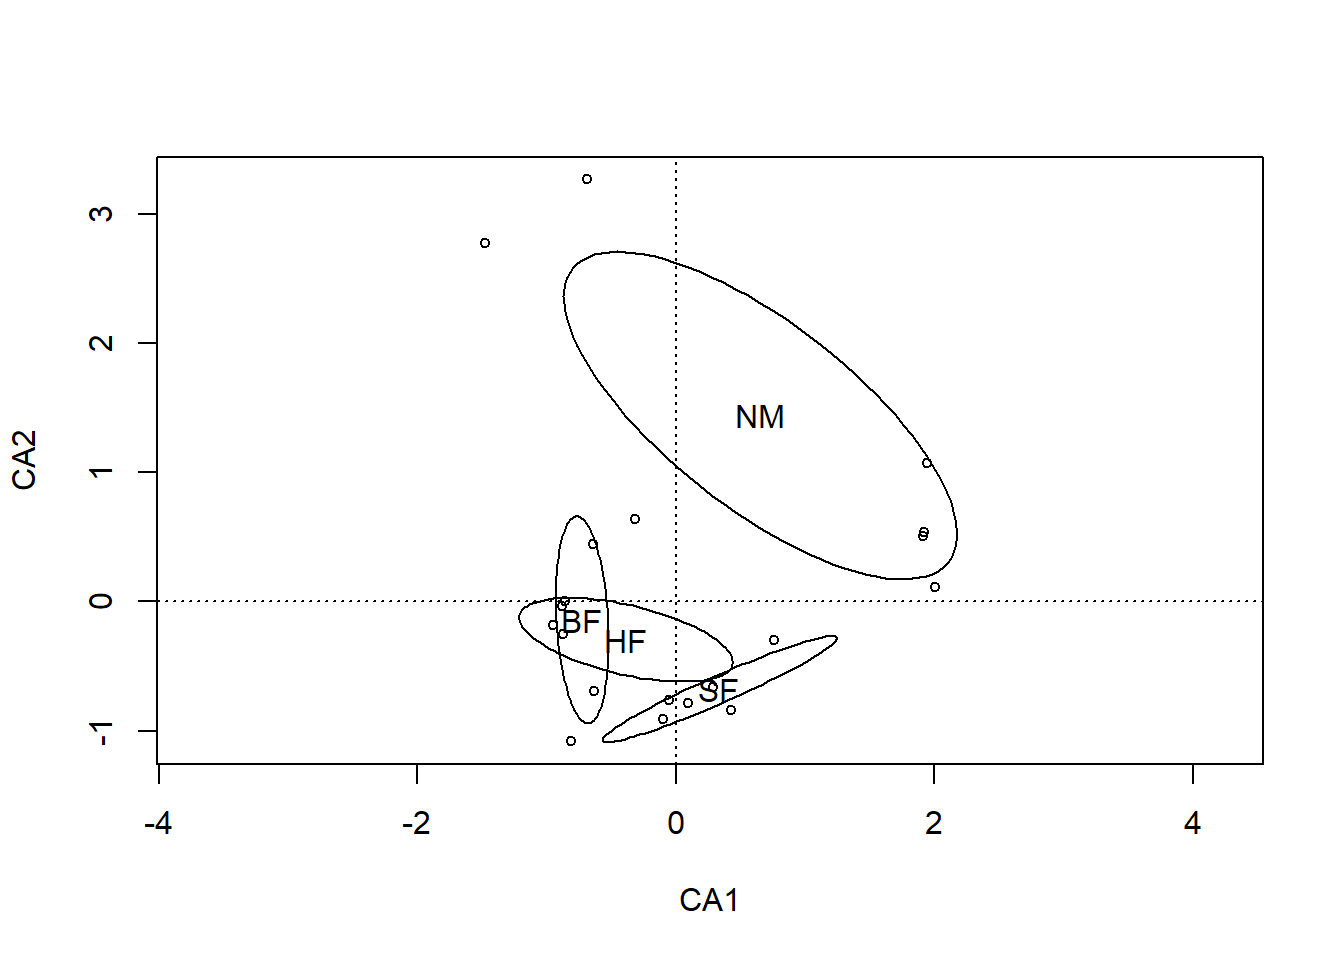
\includegraphics{AnalisisMultivarianteComunidad_files/figure-latex/unnamed-chunk-22-1.pdf}

\subsection{Ejercicio}\label{ejercicio}

Los datos que se presentan
\href{https://github.com/Ciespinosa/AnalisisMultivariante/blob/gh-pages/TraitsVege.csv}{aquí}
corresponden a rasgos asociados a procesos de dispersión de semillas,
incluyendo los potenciales grupos de dispersores. Colectamos información
de 10 rasgos de frutos y semillas de 71 especies leñosas. Se registraron
seis rasgos de frutos; tipo, color, peso, largo, ancho y número de
semillas. Para semillas se registraron tres rasgos; peso, longitud y
ancho. Adicionalmente se asignó un síndrome de dispersión a cada
especie.

Los rasgos de frutos y semillas colectados en este trabajo, han sido
asociados con la habilidad de las plantas para lidiar con el estrés.
Muller-Landau (2010) sugiere que las especies con semillas pequeñas
tienen una ventaja en fertilidad y dispersión, por producir más semillas
y facilitar su desplazamiento a grandes distancias. Por otro lado, las
semillas grandes tienen la ventaja de la tolerancia al estrés, porque
estas proveen energía y material para el crecimiento de las plántulas.
Una mayor contribución de nutrientes en semillas grandes facilita la
sobrevivencia bajo ambientes más estresantes, ya sea por sombra,
humedad, herbivoría o perturbaciones.

En este contexto, esperamos que los ambientes menos estresantes estén
dominados por especies con semillas pequeñas, pero un amplio rango de
tamaños de semillas. En ambientes de mayor estrés, se espera encontrar
un subconjunto de especies con semillas grandes y baja capacidad de
dispersión.

Para analizar el impacto del disturbio sobre la estructura de la
comunidad en términos de rasgos funcionales usaremos tres variables que
han mostrado ser un subrogado de perturbaciones antrópicas; (1)
distancia al centro poblado más cercano, (2) peso de excretas de ganado,
(3) número de árboles con DBH \textgreater{} 20 cm, donde un bajo número
de árboles grandes implica una alta perturbación. Puede obtener los
datos de
\href{https://github.com/Ciespinosa/AnalisisMultivariante/blob/gh-pages/Parcelas.csv}{aquí}

Vamos a analizar por separado los rasgos cualitativos y los
cuantitativos.

Para analizar los efectos de la perturbación sobre los rasgos
cualitativos de los frutos vamos a ajustar un PCA para cada rasgo; tipo
de fruto, síndrome de dispersión y color del fruto. Utilizaremos la
matriz de datos morfológicos cualitativos. Realizamos un modelo lineal
usando el primer eje del PCA como variable de respuesta y cada una de
las tres variables de perturbación como variables explicativas. Usaremos
la función ``rda'' del paquete ``vegan'' para ajustar el PCA, y la
función ``lm'' del paquete ``stats'' para el modelo lineal.

\section{Ordenaciones directas o
constreñidas}\label{ordenaciones-directas-o-constrenidas}

Si bien las técnicas de ordenación indirecta nos permiten descubrir
ciertos patrones, no nos permite testar hipótesis y ver las relaciones
de esta matriz con otras variables.

Si disponemos de una matriz de variables explicativas es posible
utilizar análisis de ordenación constreñidos. De esta forma, esta matriz
representa la información que tenemos sobre cada una de las muestras y
podemos usarla para predecir los valores de las variables respuesta (la
composición de especies).

Al igual que para los análisis de ordenaciones no constreñidas el tipo
de ordenación depende de la respuesta que tenemos en las variables
(Tabla \ref{tab:ordenacion1} )

\begin{table}[t]

\caption{\label{tab:ordenacion1}Relación entre el tipo de variable y el método de ordenación a utilizar}
\centering
\begin{tabular}{lll}
\toprule
Medidas.de.Similitud & Tipo.de.Ordenación & Tipo.Ordenación.Constreñida\\
\midrule
Respuesta lineal & PCA & RDA (Redundancy Analysis)\\
Respuesta Unimodal & CA/DCA & CCA (Canonical Correspondence Analysis)\\
Bray-Curtis & PcoA/mMDS/nmMDS & PERMANOVA\\
\bottomrule
\end{tabular}
\end{table}

Una interesante propiedad de los análisis de ordenación constreñidos es
que puedo hacer una ordenación parcial. Esta propiedad me permite
evaluar como un grupo de variables pueden influir en mi matriz de
respuesta. Podría dividir la información, por ejemplo, en variables
ambientales y variables bióticas y ver cuánto explica cada una y cuanto
explican en conjunto.

\section{Realizando una ordenación
constreñida}\label{realizando-una-ordenacion-constrenida}

Al igual que en el caso de la ordenación no constreñida debemos decidir
el tipo de ordenación constreñida que vamos hacer. En el caso de los
datos de \emph{Dune} sabemos que la respuesta es unimodal por lo que
escogeremos un análisis canónico de correspondencias (CCA) para nuestra
ordenación constreñida.

Para hacer la ordenación constreñida necesitamos una matriz con
variables explicativas, utilizaremos las variables provistas en el
paquete vegan denominadas env.env.

\begin{Shaded}
\begin{Highlighting}[]
\KeywordTok{data}\NormalTok{(}\StringTok{"dune.env"}\NormalTok{) }\CommentTok{#Llamamos a los datos}

\NormalTok{ord.cca <-}\StringTok{ }\KeywordTok{cca}\NormalTok{(dune~}\StringTok{ }\NormalTok{A1 +}\StringTok{ }\NormalTok{Use, }\DataTypeTok{data=}\NormalTok{dune.env)}
\NormalTok{ord.cca}
\end{Highlighting}
\end{Shaded}

\begin{verbatim}
## Call: cca(formula = dune ~ A1 + Use, data = dune.env)
## 
##               Inertia Proportion Rank
## Total          2.1153     1.0000     
## Constrained    0.4724     0.2233    3
## Unconstrained  1.6429     0.7767   16
## Inertia is scaled Chi-square 
## 
## Eigenvalues for constrained axes:
##    CCA1    CCA2    CCA3 
## 0.27630 0.14929 0.04683 
## 
## Eigenvalues for unconstrained axes:
##    CA1    CA2    CA3    CA4    CA5    CA6    CA7    CA8    CA9   CA10 
## 0.3792 0.3091 0.2093 0.1629 0.1308 0.0965 0.0758 0.0731 0.0483 0.0456 
##   CA11   CA12   CA13   CA14   CA15   CA16 
## 0.0431 0.0237 0.0163 0.0141 0.0108 0.0042
\end{verbatim}

Lo que podemos ver es que la variable A1 más Use explican el 22.33\% de
la variación en los datos.

La decisión de que modelos deberían generar debe responder a una lógica
ecológica, así podemos probar como algunas variables juegan o no un rol
en la estructura de la comunidad.

Una herramienta que podríamos utilizar para analizar la importancia de
cada variable es utilizar la función \texttt{envfit}, esta función
permite relacionar la ordenación no constreñida con las variables
explicativas y mediante un test de permutación mostrarnos que variables
se asocian significativamente con la ordenación.

\begin{Shaded}
\begin{Highlighting}[]
\NormalTok{fitVar <-}\StringTok{ }\KeywordTok{envfit}\NormalTok{(ord.cca, dune.env)}
\NormalTok{fitVar}
\end{Highlighting}
\end{Shaded}

\begin{verbatim}
## 
## ***VECTORS
## 
##         CCA1      CCA2     r2 Pr(>r)  
## A1  0.996690 -0.081278 0.4812  0.011 *
## ---
## Signif. codes:  0 '***' 0.001 '**' 0.01 '*' 0.05 '.' 0.1 ' ' 1
## Permutation: free
## Number of permutations: 999
## 
## ***FACTORS:
## 
## Centroids:
##                 CCA1    CCA2
## Moisture1    -0.7841  0.1023
## Moisture2    -0.7047 -0.3941
## Moisture4    -0.0690 -1.1244
## Moisture5     1.4052  0.5459
## ManagementBF -0.8428  0.0317
## ManagementHF -0.3461 -0.1831
## ManagementNM  0.9747  2.0835
## ManagementSF  0.1233 -1.3692
## UseHayfield  -0.3809  1.2869
## UseHaypastu  -0.1953 -1.0131
## UsePasture    0.8511 -0.0640
## Manure0       0.9747  2.0835
## Manure1      -0.5822  0.0043
## Manure2      -0.5826 -0.3399
## Manure3       0.6233 -0.6456
## Manure4      -0.7009 -1.5898
## 
## Goodness of fit:
##                r2 Pr(>r)    
## Moisture   0.3176  0.035 *  
## Management 0.4941  0.001 ***
## Use        0.3204  0.005 ** 
## Manure     0.5105  0.001 ***
## ---
## Signif. codes:  0 '***' 0.001 '**' 0.01 '*' 0.05 '.' 0.1 ' ' 1
## Permutation: free
## Number of permutations: 999
\end{verbatim}

Podemos utilizar el \emph{Goodness of fit} para ver cuáles son las
variables que ajustan la ordenación y utilizar estas para hacer el
modelo constreñido. En este caso utilizaremos Manure y Management.

\begin{Shaded}
\begin{Highlighting}[]
\NormalTok{ord.ccafit <-}\StringTok{ }\KeywordTok{cca}\NormalTok{(dune~Manure+Management, }\DataTypeTok{data=}\NormalTok{dune.env)}
\NormalTok{ord.ccafit}
\end{Highlighting}
\end{Shaded}

\begin{verbatim}
## Call: cca(formula = dune ~ Manure + Management, data = dune.env)
## 
##               Inertia Proportion Rank
## Total          2.1153     1.0000     
## Constrained    0.8766     0.4144    6
## Unconstrained  1.2386     0.5856   13
## Inertia is scaled Chi-square 
## Some constraints were aliased because they were collinear (redundant)
## 
## Eigenvalues for constrained axes:
##   CCA1   CCA2   CCA3   CCA4   CCA5   CCA6 
## 0.3617 0.2271 0.1454 0.0655 0.0418 0.0353 
## 
## Eigenvalues for unconstrained axes:
##    CA1    CA2    CA3    CA4    CA5    CA6    CA7    CA8    CA9   CA10 
## 0.4082 0.1592 0.1493 0.1252 0.0962 0.0774 0.0649 0.0424 0.0382 0.0312 
##   CA11   CA12   CA13 
## 0.0251 0.0121 0.0090
\end{verbatim}

Como vemos con este procedimiento subimos al 41\% de la varianza
explicada.

Podemos utilizar la función anova para evaluar la significancia de cada
variable dentro del modelo, de forma separada.

\begin{Shaded}
\begin{Highlighting}[]
\NormalTok{ord.ccaT <-}\StringTok{ }\KeywordTok{cca}\NormalTok{(dune~}\StringTok{ }\NormalTok{., }\DataTypeTok{data=}\NormalTok{dune.env)}
\KeywordTok{anova}\NormalTok{(ord.ccaT, }\DataTypeTok{by=}\StringTok{"term"}\NormalTok{, }\DataTypeTok{permu=}\DecValTok{1000}\NormalTok{)}
\end{Highlighting}
\end{Shaded}

\begin{verbatim}
## Permutation test for cca under reduced model
## Terms added sequentially (first to last)
## Permutation: free
## Number of permutations: 999
## 
## Model: cca(formula = dune ~ A1 + Moisture + Management + Use + Manure, data = dune.env)
##            Df ChiSquare      F Pr(>F)  
## A1          1   0.22476 2.5704  0.014 *
## Moisture    3   0.51898 1.9783  0.014 *
## Management  3   0.39543 1.5074  0.072 .
## Use         2   0.10910 0.6238  0.926  
## Manure      3   0.25490 0.9717  0.528  
## Residual    7   0.61210                
## ---
## Signif. codes:  0 '***' 0.001 '**' 0.01 '*' 0.05 '.' 0.1 ' ' 1
\end{verbatim}

Como vemos esto cambia lo que inicialmente habíamos decidido, esto es
debido a que algunas de las variables pueden estar correlacionadas entre
ellas.

Bien ahora necesitamos graficar los resultados. Podemos utilizar la
función plot e ir graficando cada uno de los componentes (Figura
\ref{fig:plotcca}).

\begin{Shaded}
\begin{Highlighting}[]
\KeywordTok{plot}\NormalTok{(ord.cca, }\DataTypeTok{dis=}\StringTok{"sp"}\NormalTok{, }\DataTypeTok{type=}\StringTok{"n"}\NormalTok{)}
\KeywordTok{points}\NormalTok{(ord.cca, }\DataTypeTok{dis=}\StringTok{"sites"}\NormalTok{, }\DataTypeTok{pch=}\DecValTok{19}\NormalTok{, }\DataTypeTok{col=}\StringTok{"grey"}\NormalTok{)}
\KeywordTok{points}\NormalTok{(ord.cca, }\DataTypeTok{display=}\StringTok{"cn"}\NormalTok{, }\DataTypeTok{col=}\StringTok{"blue"}\NormalTok{, }\DataTypeTok{pch=}\DecValTok{19}\NormalTok{)}
\KeywordTok{text}\NormalTok{(ord.cca, }\DataTypeTok{dis=}\StringTok{"sp"}\NormalTok{, }\DataTypeTok{cex=}\FloatTok{0.6}\NormalTok{)}
\KeywordTok{text}\NormalTok{(ord.cca, }\DataTypeTok{display =} \StringTok{"cn"}\NormalTok{, }\DataTypeTok{col=}\StringTok{"blue"}\NormalTok{, }\DataTypeTok{cex=}\FloatTok{0.7}\NormalTok{)}
\end{Highlighting}
\end{Shaded}

\begin{figure}

{\centering 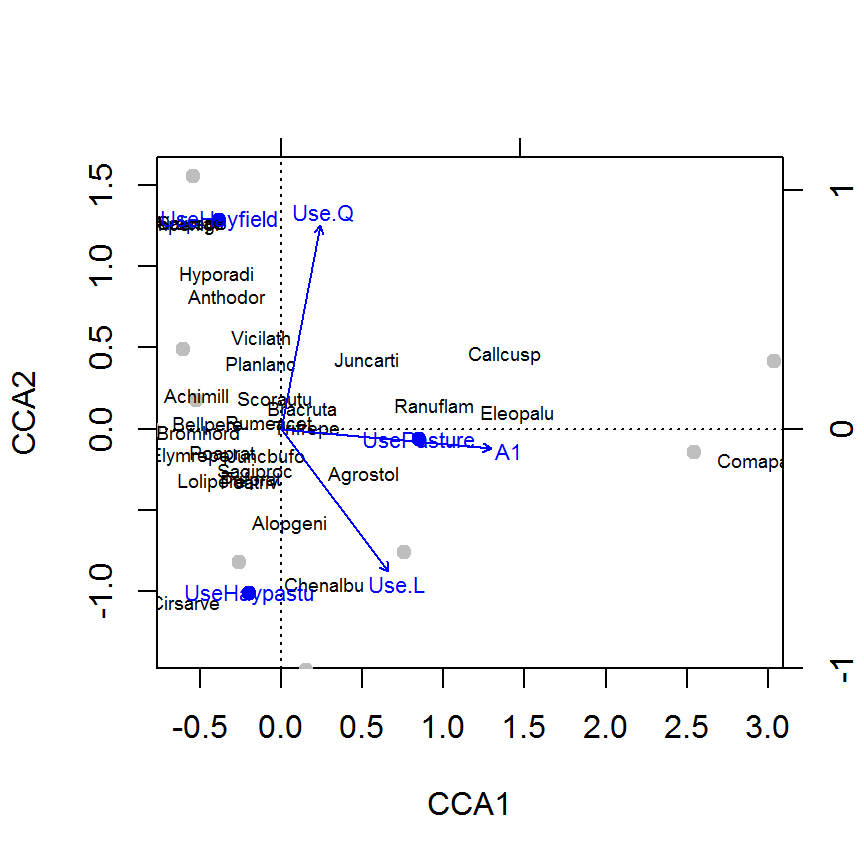
\includegraphics{AnalisisMultivarianteComunidad_files/figure-latex/plotcca-1} 

}

\caption{Representación gráfica del CCA}\label{fig:plotcca}
\end{figure}

Muchas veces uno de los problemas que tenemos para graficar los datos es
que los nombres de las especies son muy largos, en estos casos podemos
utilizar una función que se denomina \texttt{make.cepnames} la cual
permite acortar los nombres.

\begin{Shaded}
\begin{Highlighting}[]
\KeywordTok{data}\NormalTok{(BCI)}
\KeywordTok{names}\NormalTok{(BCI[}\DecValTok{1}\NormalTok{:}\DecValTok{5}\NormalTok{])}
\end{Highlighting}
\end{Shaded}

\begin{verbatim}
## [1] "Abarema.macradenia"    "Vachellia.melanoceras" "Acalypha.diversifolia"
## [4] "Acalypha.macrostachya" "Adelia.triloba"
\end{verbatim}

\begin{Shaded}
\begin{Highlighting}[]
\NormalTok{short <-}\StringTok{ }\KeywordTok{make.cepnames}\NormalTok{(}\KeywordTok{names}\NormalTok{(BCI[}\DecValTok{1}\NormalTok{:}\DecValTok{5}\NormalTok{]))}
\NormalTok{short}
\end{Highlighting}
\end{Shaded}

\begin{verbatim}
## [1] "Abarmacr" "Vachmela" "Acaldive" "Acalmacr" "Adeltril"
\end{verbatim}

Existen procedimientos para construir modelos que ahora no tocaremos,
puede encontrar más información en
\href{http://cc.oulu.fi/~jarioksa/opetus/metodi/vegantutor.pdf}{Oksanen
2015}

Nota: para realizar un permanova debemos utilizar la función adonis. El
procedimiento es similar al desarrollo del cca.

\section{Ejercicio 3: Análisis de
Ordenación}\label{ejercicio-3-analisis-de-ordenacion}

Con los datos utilizados para realizar el análisis de aglomerados, vamos
a realizar un análisis de ordenación constreñida.

\begin{enumerate}
\def\labelenumi{\alph{enumi}.}
\item
  Defina que tipo de ordenación constreñida debe realizar para explicar
  la variación de los datos de herbáceas.
\item
  Realice un análisis para definir las variables que se debería utilizar
  en el análisis
\item
  Ajuste un modelo y defina el porcentaje de variación explicado.
\item
  Compara los resultados de la ordenación directa si en vez de
  transformar los datos corremos los modelos con los datos brutos.
\item
  Realice un gráfico del modelo desarrollado.
\end{enumerate}

\bibliography{packages.bib}


\end{document}
